\clearpage
\chapter{Machine Learning}\label{sec:machinelearning}
ROIs are artificial regions created by the CMSSW mechanism, displaced vertex candidates.
ROIs contain thorough information about fitted tracks, vertices, and isolation, following the formation procedure described in the previous section.
The exhaustive variables saved in each ROI contain information that directly and indirectly tells whether the ROI is from the signal or background process.
Given the extensive amount of variables within ROIs, it is inappropriate to use ROIs' single or a few variables as our tagging variables, like in ZH analysis ~\cite{ZHAN}.
It is also inefficient to implement a cut-based approach due to having so many variables from ROI.
The optimization process for all these vertex, isolation, and track variables would be extremely time-consuming, inefficient, and error-prone.
Therefore, the analysis exploits machine learning (ML) for this multivariate analysis.
Boosted decision trees will also face a similar problem as cut-based analysis, although somewhat.
Deep Neural networks are the most adaptable ML algorithm for this analysis method, in which the algorithm inputs an extensive list of ROI variables into a neural network and receives a final score to discriminate ROIs that arise in signal process versus background processes.
The list of variables inputted into the ML algorithms is provided in subsection \ref{sec:MLIV}.

The analysis uses Keras-Tensorflow for its ML platform.
CMSSW includes Keras-Tensorflow, which enables simple and easy usage of Keras-Tensorflow with simple commands in various CMS remote clusters.
For CMSSW\_10\_6\_12 (to have access to the B Parking trigger path), the Keras-Tensorflow version is 2.3.1.
It runs with CPUs and GPUs.
\section{Machine Learning Input Variables}\label{sec:MLIV}
As discussed in chapter \ref{sec:objects}, the ROI has vertex and shell (isolation) information.
Vertex information is trained with 19 different variables, which are listed and categorized in Tables ~\ref{tab:ROITCvars}.
%, ~\ref{tab:ROIANvars}, and ~\ref{tab:ROIEVvars}.

\begin{table}[htb]
\caption{ROI (trackCluster) variables by category}
\begin{center}
\begin{tabular}{r|l|l}\hline
 TrackCluster & Position & TrackClusters.vx() - primaryVertex.X() \\
              & Position & TrackClusters.vy() - primaryVertex.Y() \\
              & Position & TrackClusters.vz() - primaryVertex.Z() \\
              & Covariance & TrackClusters.vertexCovariance()(0,0) \\
              & Covariance & TrackClusters.vertexCovariance()(0,1) \\
              & Covariance & TrackClusters.vertexCovariance()(0,2) \\
              & Covariance & TrackClusters.vertexCovariance()(1,0) \\
              & Covariance & TrackClusters.vertexCovariance()(1,1) \\
              & Covariance & TrackClusters.vertexCovariance()(1,2) \\
              & Track0,1 & Track0,1.pt \\
              & Track0,1 & Track0,1.eta \\
              & Track0,1 & Track0,1.phi \\
              & Track0,1 & Track0,1.dxy \\
              & Track0,1 & Track0,1.dz \\
              & Track0,1 & Track0,1.normalizedChi2 \\
              & Track0,1 & Track0,1.HighPurityInt \\
 \hline
 \hline
\end{tabular}
\label{tab:ROITCvars}
\end{center}
\end{table}



Shell information is trained with 8 different variables, which are listed in Tables ~\ref{tab:ROIANvars}.

\begin{table}[htb]
\caption{ROI (Annulus) variables by category}
\begin{center}
\begin{tabular}{r|l|l}\hline
 Annulus      & pfCandidate/LostTracks & pfCandidate/LostTracks.pt \\
              & pfCandidate/LostTracks & pfCandidate/LostTracks.eta \\
              & pfCandidate/LostTracks & pfCandidate/LostTracks.phi \\
              & pfCandidate/LostTracks & pfCandidate/LostTracks.dxy \\
              & pfCandidate/LostTracks & pfCandidate/LostTracks.dz \\
              & pfCandidate/LostTracks & pfCandidate/LostTracks.normalizedChi2 \\
              & pfCandidate/LostTracks & pfCandidate/LostTracks.HighPurityInt \\
              & pfCandidate/LostTracks & pfCandidate/LostTracks.$\Delta$R(trackMomentum) \\
 \hline
 \hline
\end{tabular}
\label{tab:ROIANvars}
\end{center}
\end{table}

We input vertex and shell information into separate ML networks. Thus, we get two final products from the ML networks, one for the vertex information and the other for the shell information.

 \begin{figure}[h!]
   \caption{Simple cartoon showing ML network for vertex and annulus shell.}
   \label{fig:NetworkML}
   \centering
   \includegraphics[width=0.6\linewidth]{figs/PhiVNet.png}
   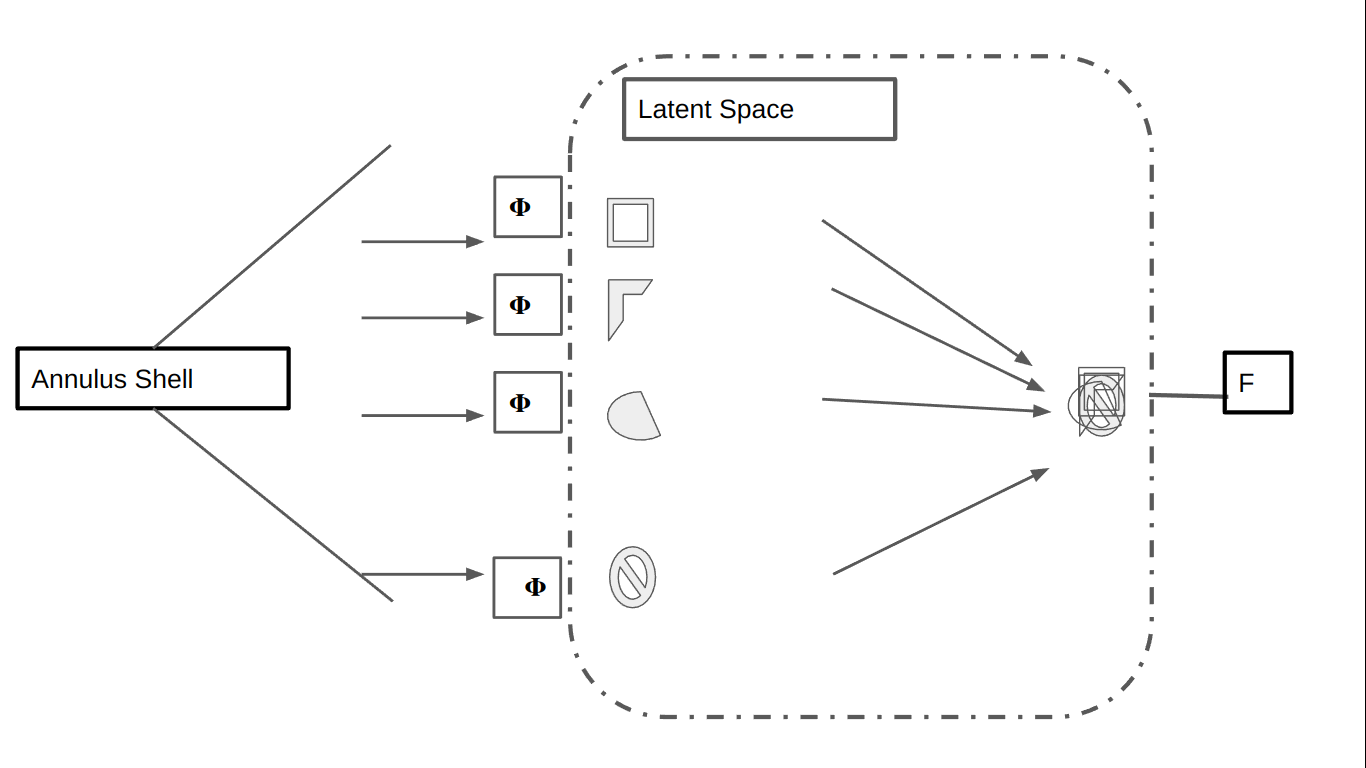
\includegraphics[width=0.6\linewidth]{figs/PhiANet.png}
 \end{figure}

%\begin{table}[htb]
%\caption{Event variables by category}
%\begin{center}
%\begin{tabular}{r|l|l}\hline
%  ROI    & Position & x \\
%         & Position & y \\
%         & Position & z \\
% \hline
% \hline
%\end{tabular}
%\label{tab:ROIEVvars}
%\end{center}
%\end{table}

\section{Fine-Tuning of ML environemnt}
CMSSW includes an image container for Keras-Tensorflow, and researchers can also submit remote batch jobs for its ML training.
The analysis tested multiple variables (such as epoch numbers, batch sizes, phi sizes, and f sizes) of our DNN layers thanks to the submission of remote batch jobs with CMSSW's Keras-Tensorflow image container.
The analysis tested different signal vs. background dataset combinations for maximum discriminant power.
The list of mass scale and lifetime tested for signal points are listed in the appendix.
Different SM physics process (and their compositions) tested for background process are also listed in the appendix.

The final Tensorflow product used for the analysis was trained with parameters in the following section.
Keras-Tensorflow DNN variable information was fine-tuned with these variables for the maximum Area Under the Curve (AUC) value.
Its information is listed in the table \ref{tab:ROIParam}.
\begin{table}[htb]
\caption{Parameters for ML network}
\begin{center}
\begin{tabular}{r|l}\hline
Epoch & 300 \\
batch size & 250 \\
Phi sizes & (64,128,256) for vertex ,(32,64,128) for shell \\
f sizes & (256,128,32) \\
Signal & ggHSSTo4Tau-MS15GeV-c$\tau$100mm  \\
Background & QCD\_Pt120-170\_MuEneriched and TTJets \\
 \hline
 \hline
\end{tabular}
\label{tab:ROIParam}
\end{center}
\end{table}


\section{ML scores of the ROIs}
More than 10 ROIs per event often exist from our ROI reconstruction mechanism.
However, we do not need all ROIs per event, as most of them are low-scoring ROIs that came from track misconstruction and others.
The signal process has two scalar decays as in Figure~\ref{fig:feynmanggH}, and it is reasonable to use only the two highest-scoring ROIs for our analysis.
Thus, we define the leading ROI (leadROI) as an ROI with the highest vertex score in the event.
Likewise, it would be easy to define the subleading ROI (subleadROI) as an ROI with the second highest vertex score in the event.
However, the subleadROI is not simply the second highest-scoring ROI of the event due to the non-negligible lifetime of $\tau$ leptons in the detector.
After obtaining an ROI with the highest ML vertex score, we search for the next highest scored ROI, $\Delta\Phi$>0.4, from the leading ROI to avoid counting ROI from the same LLP decay.
The ordering is done by vertex discriminant since it is more potent than the shell discriminant.
For better numerical representation, we use log base 10 value of ROI vertex score subtracted from 1.
Mathmatical definition of loglead and logexclead are in formulae \ref{eq:log} and \ref{eq:logexc}. 
\begin{equation}
\label{eq:log}
	loglead = Log10(1-ROI's\;leading\;Vertex\;score)
\end{equation}
\begin{equation}
\label{eq:logexc}
	logexclead = Log10(1-ROI's\;subleading\;Vertex\;score),\;with\;\Delta\Phi(lead,sublead) \geq 0.4.
\end{equation}
%More detailed explanations are described in section~\ref{sec:lifetimeROI}.)  
%The cuts on the leading ROI, and the subleading ROI are optimized based on maximizing the punzi significance formula with value $\sigma$ set to discovery value of 5.  
%\begin{equation}\label{eq:significance}
%    \sigma(N_{\mathrm{displaced-tag}}) = \frac{S(N_{\mathrm{displaced-tag}})} {\sqrt{B(N_{\mathrm{displaced-tag}})} + 2.5 }.
%\end{equation}

%\begin{figure}[h!]
%  \caption{Tensorflow scores}
%  \label{fig:TensorFlow scores}
%  \centering
%  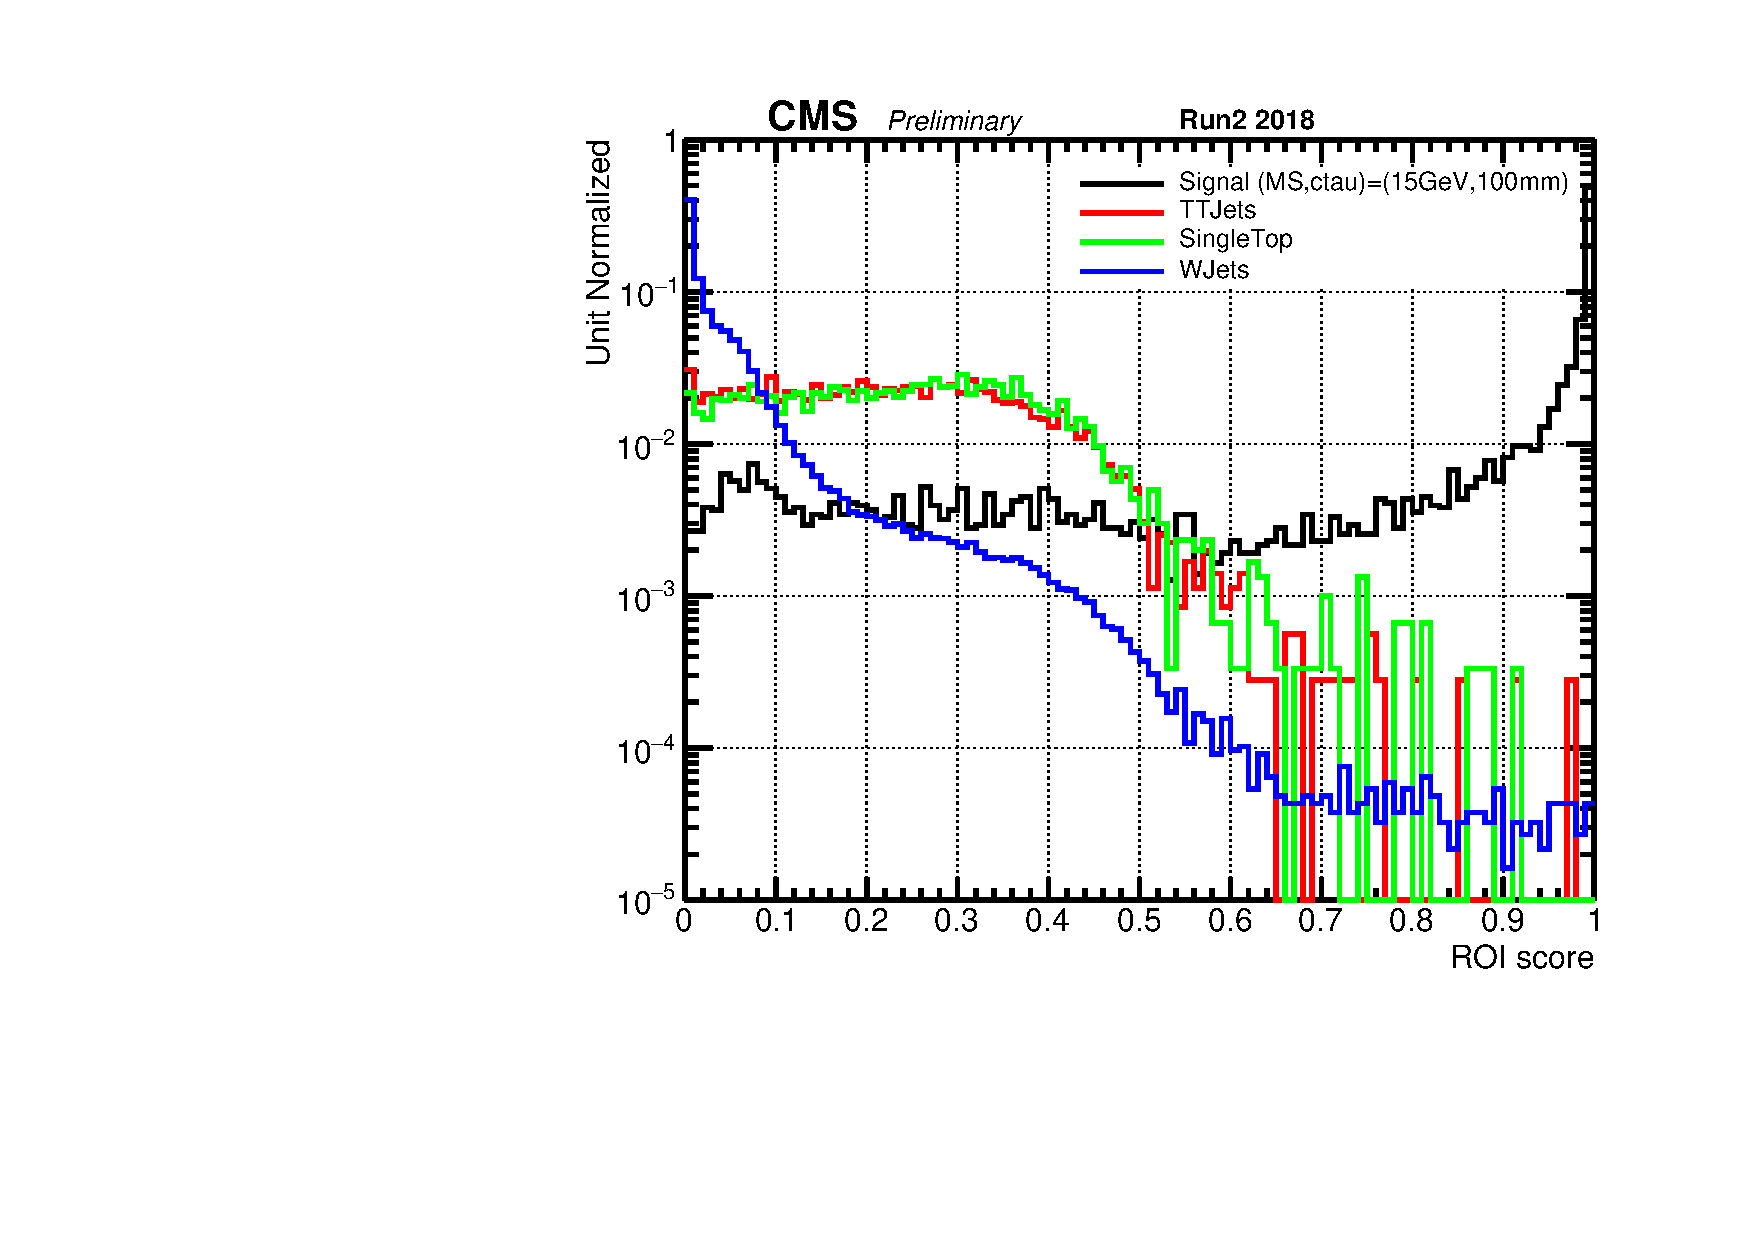
\includegraphics[width=0.67\linewidth]{figs/Tensorflow_Disc_mostrecent.pdf}
%
%\end{figure}

 \begin{figure}[h!]
   \caption{Signal versus Background for loglead, where the ROI score is the highest ROI of the event. Left plot is for MS-15\_ctauS-10mm point, whereas the right plot is for MS-15\_cauS-100mm point}
   \label{fig:leadROIscore}
   \centering
   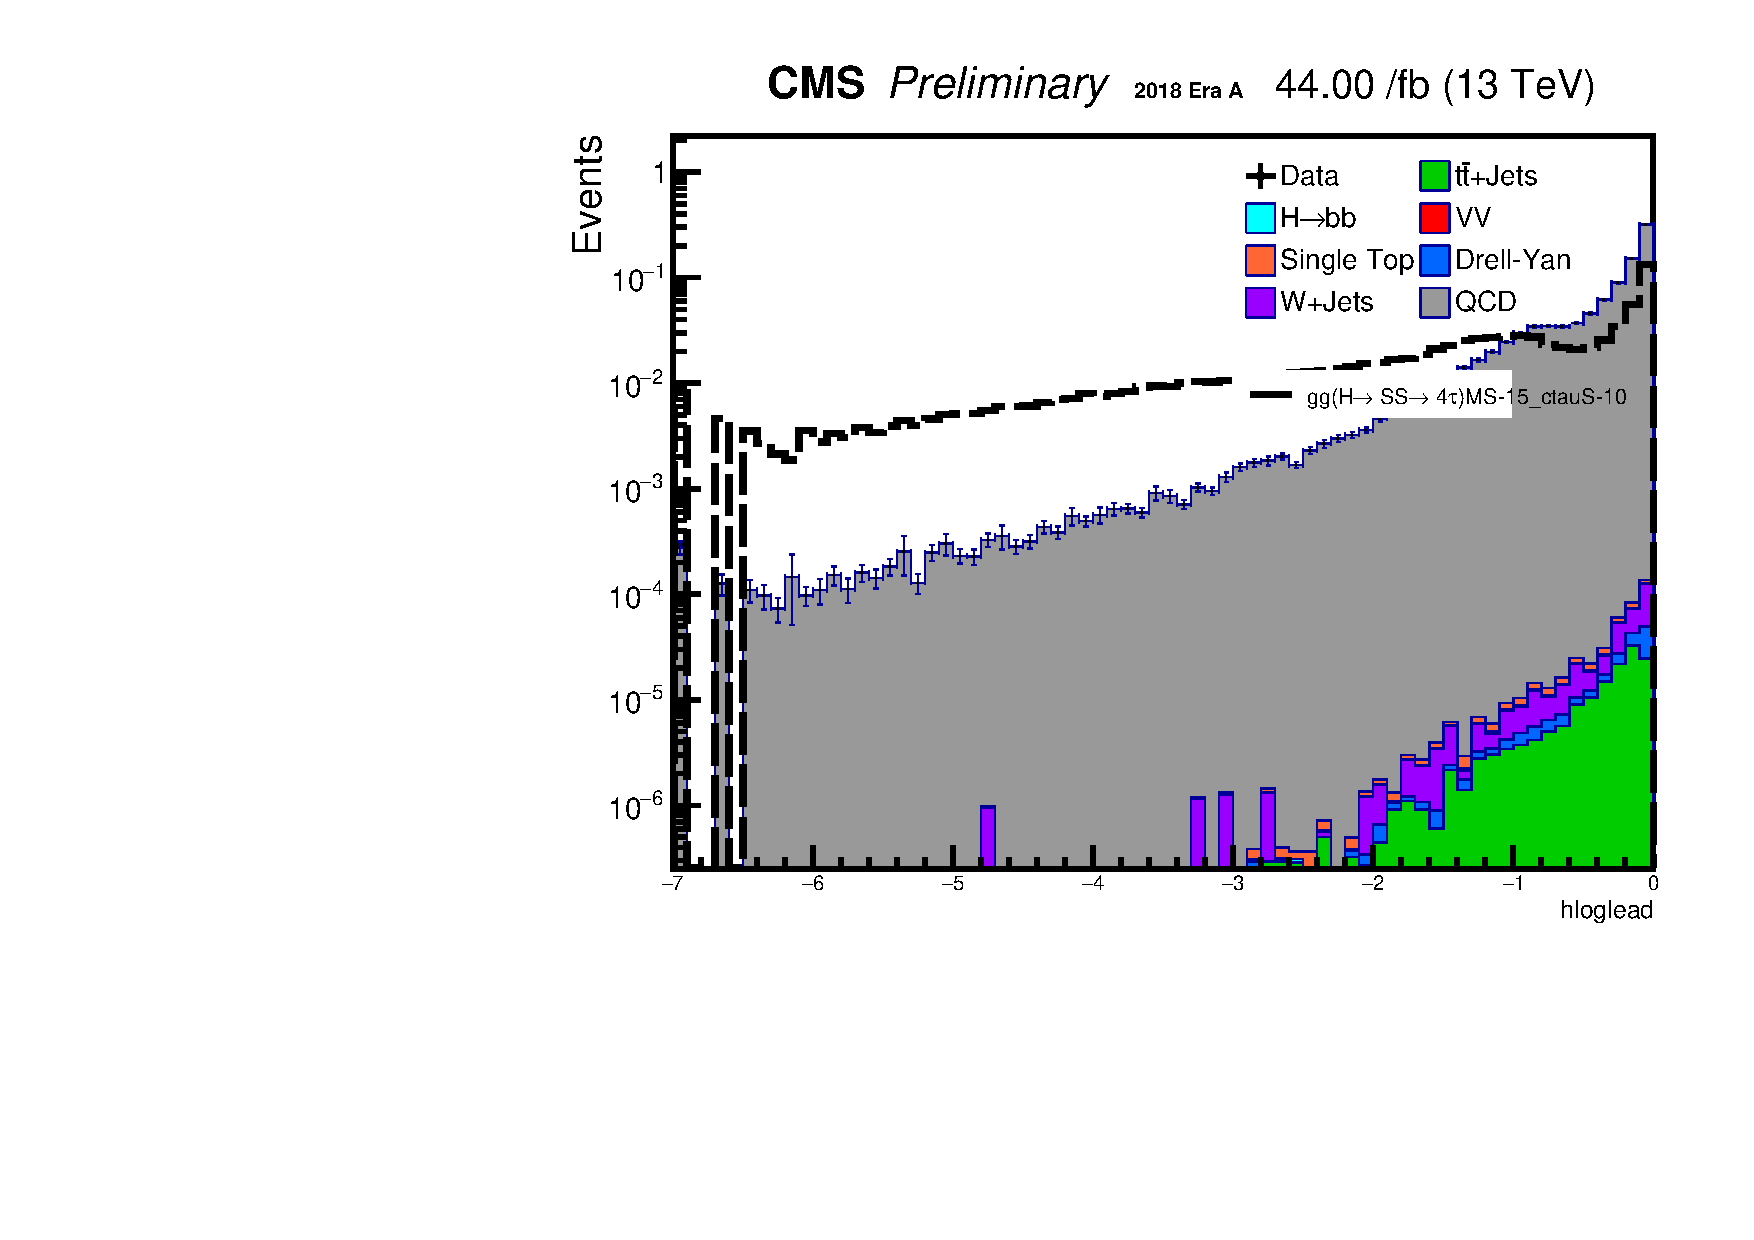
\includegraphics[width=0.47\linewidth]{figs/log_AnalysisNote_MS-15_ctauS-10_hloglead.pdf}
   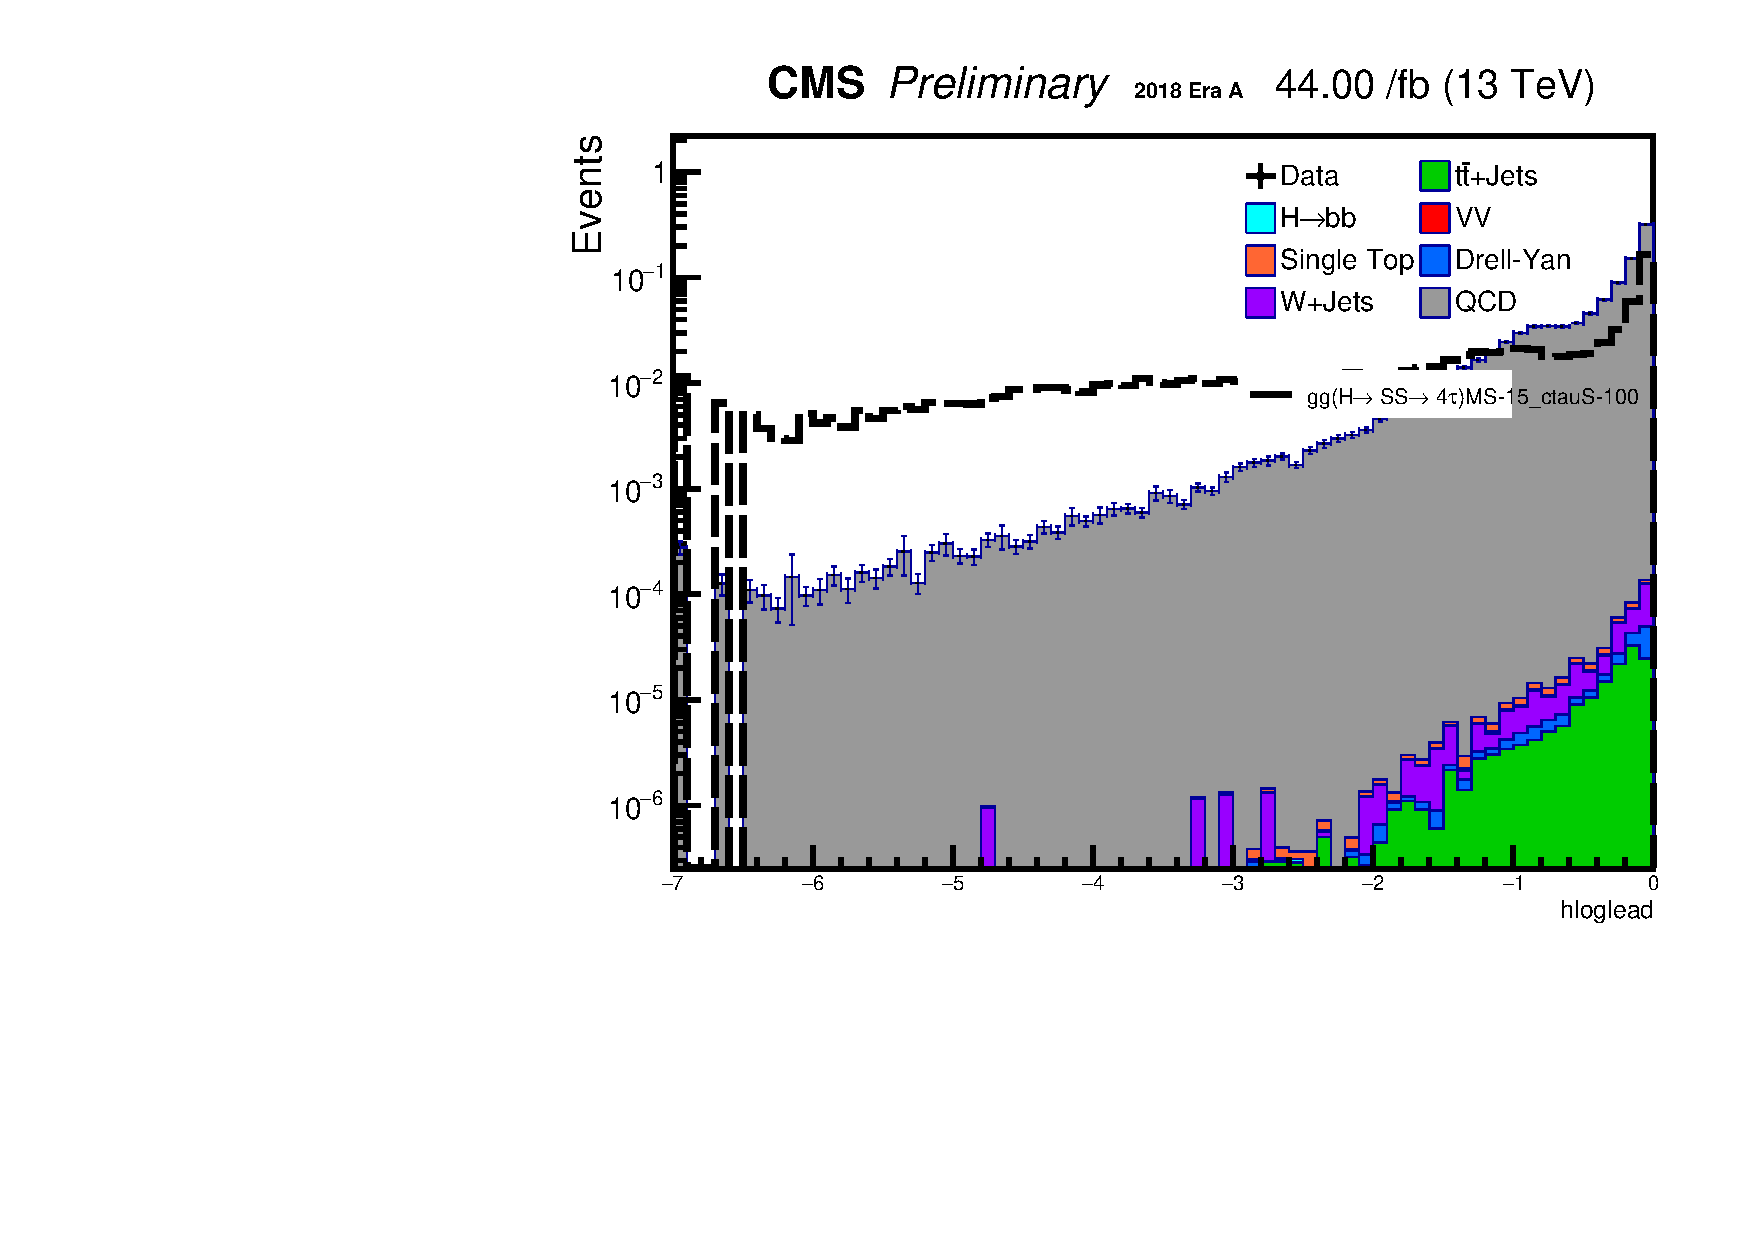
\includegraphics[width=0.47\linewidth]{figs/log_AnalysisNote_MS-15_ctauS-100_hloglead.pdf}
   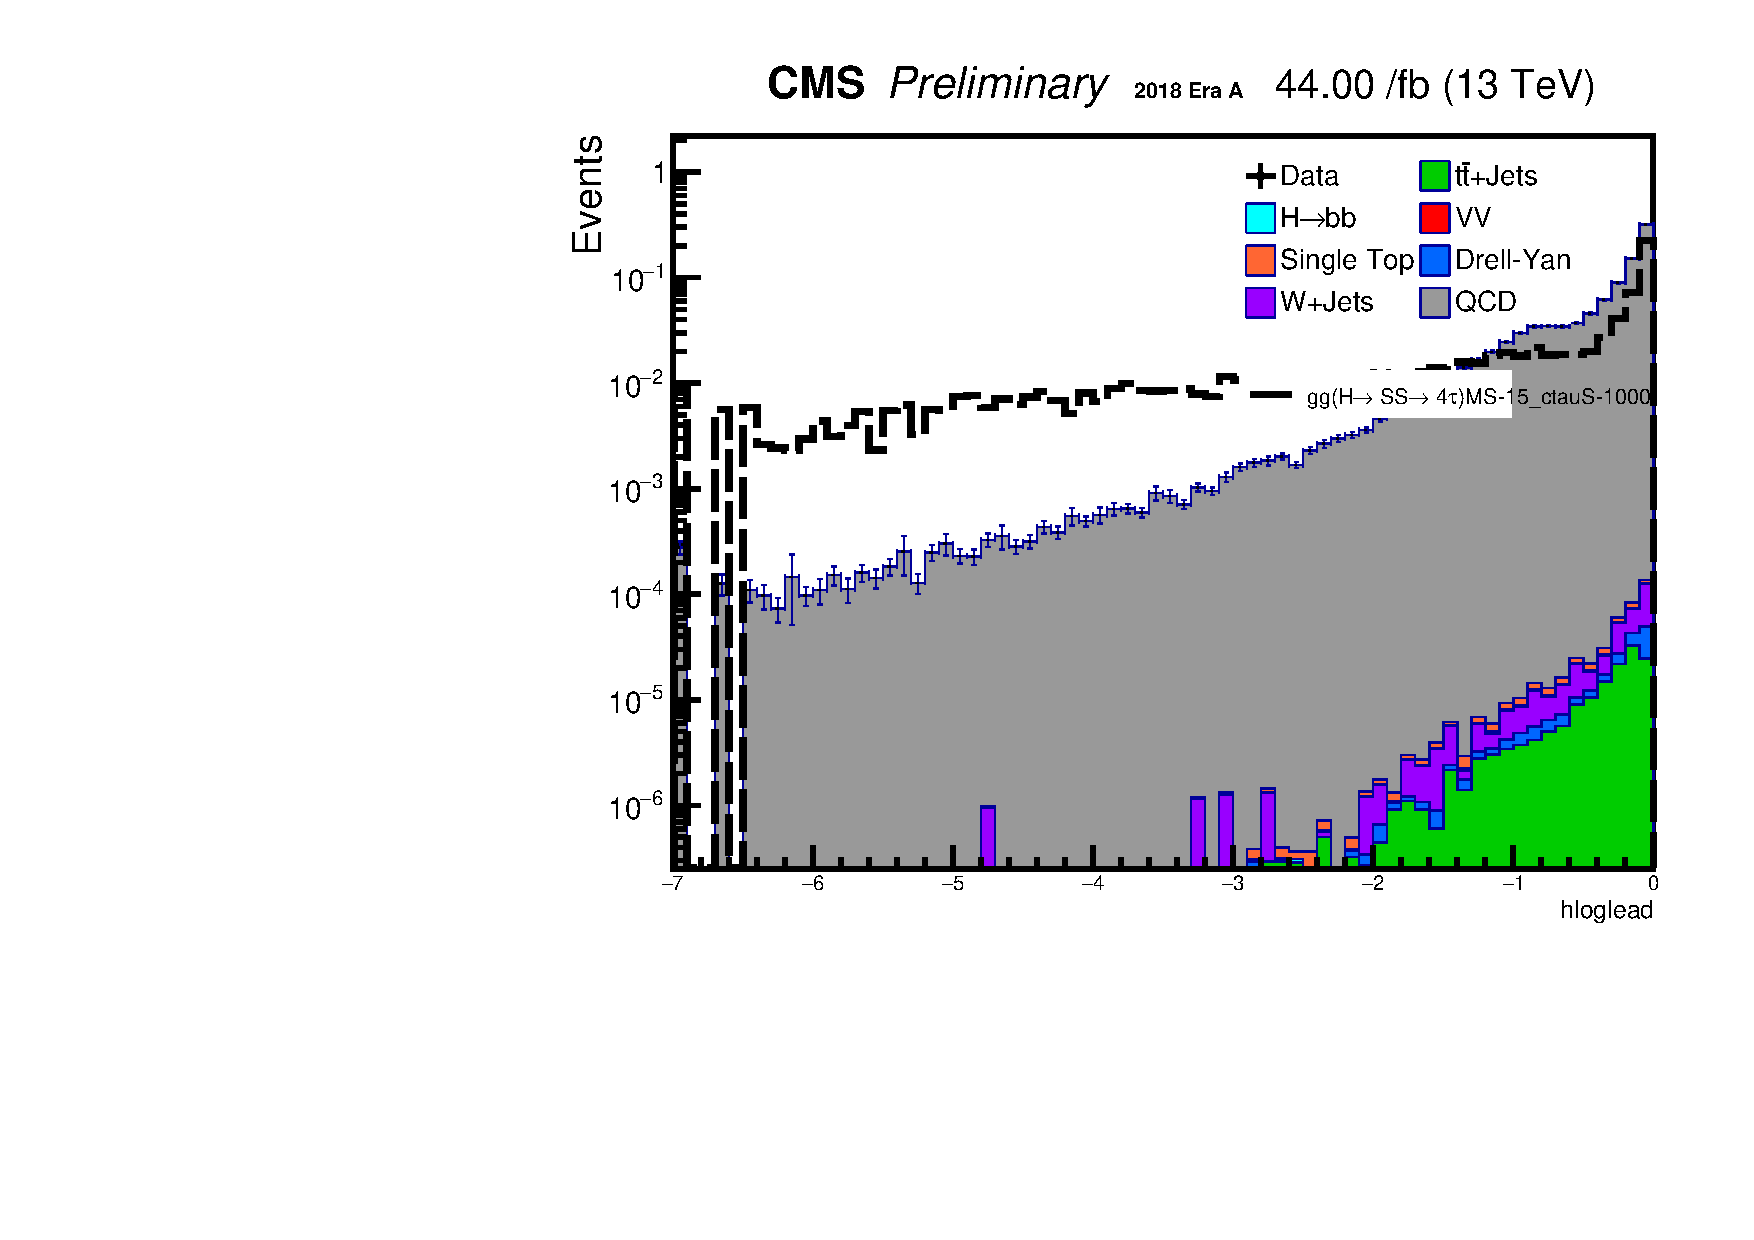
\includegraphics[width=0.47\linewidth]{figs/log_AnalysisNote_MS-15_ctauS-1000_hloglead.pdf}
   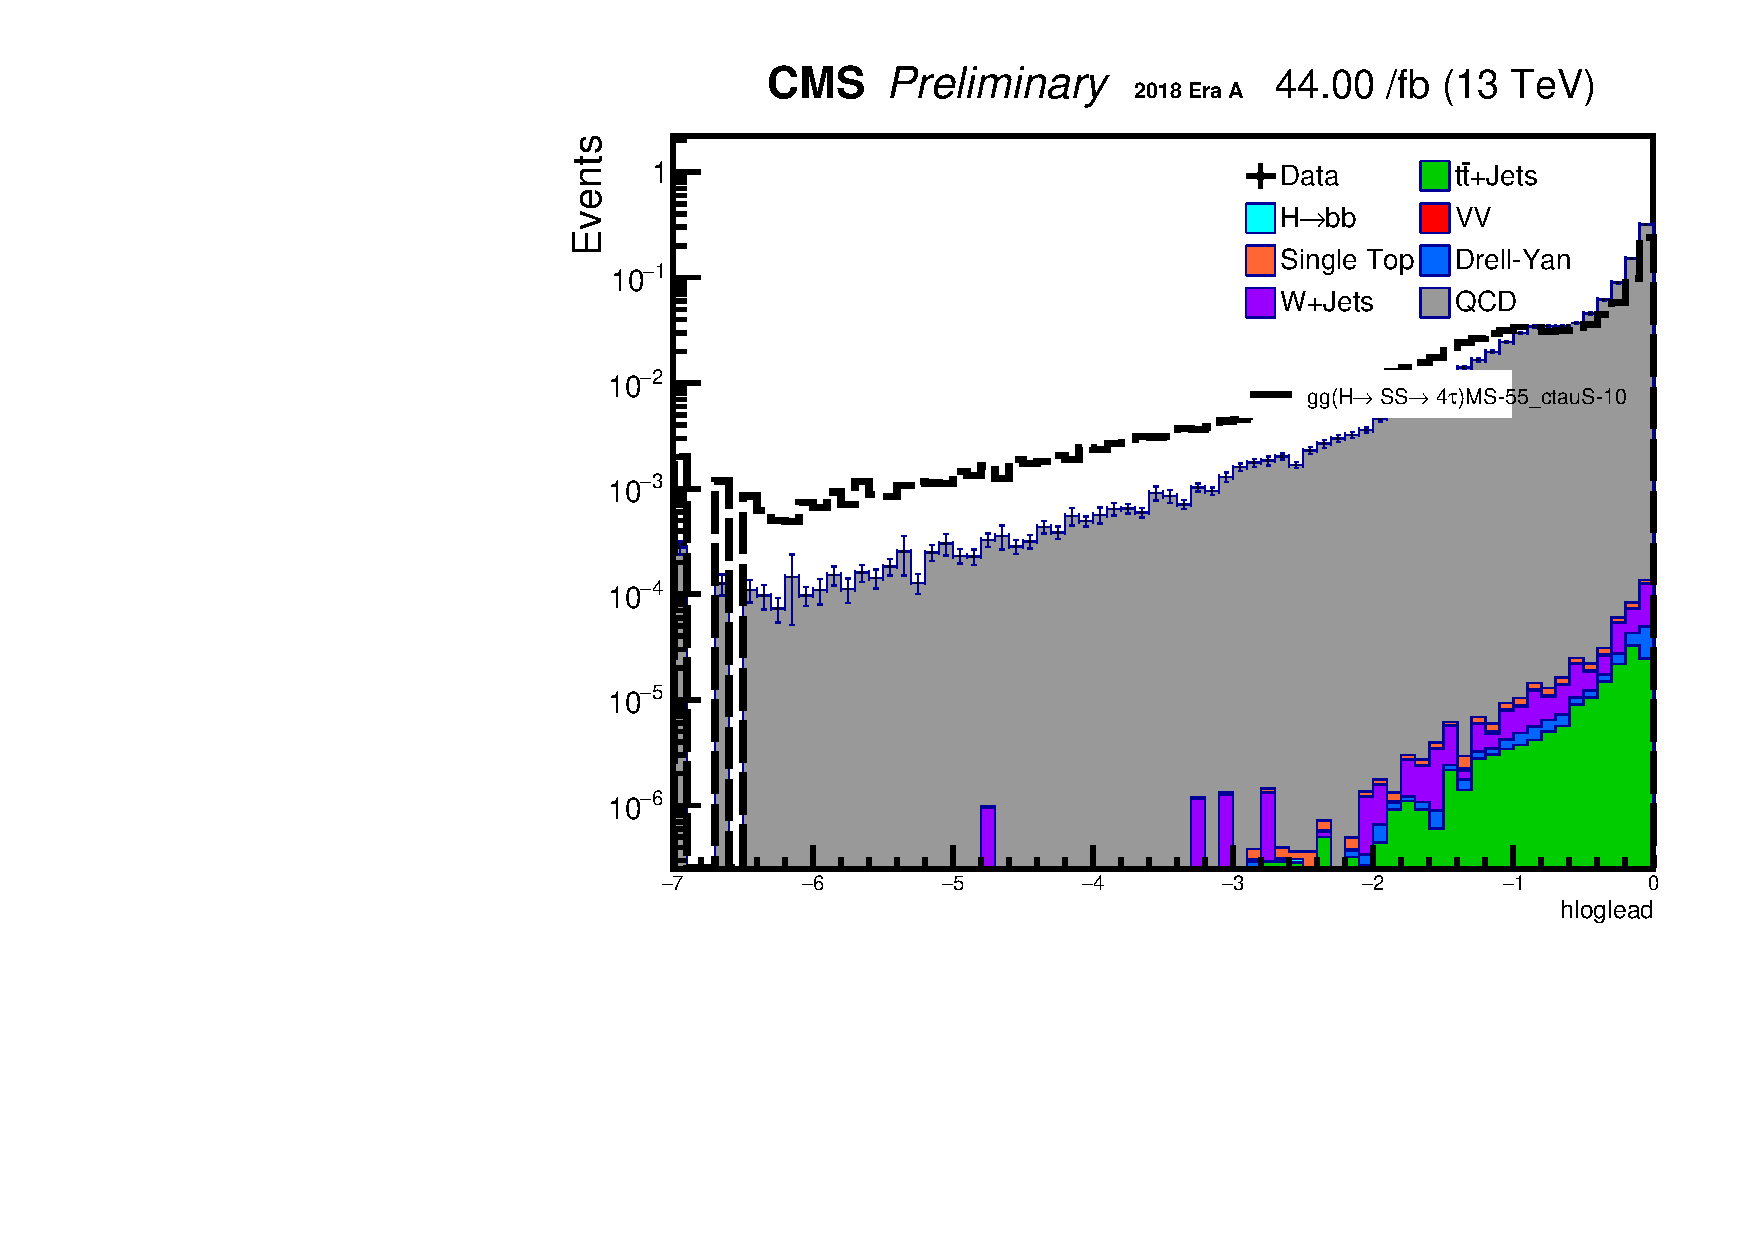
\includegraphics[width=0.47\linewidth]{figs/log_AnalysisNote_MS-55_ctauS-10_hloglead.pdf}
 \end{figure}


 \begin{figure}[h!]
	 \caption{Signal versus Background for logexclead (sublead), where the ROI score is the second highest ROI (outside of dPhi=0.4 from leading ROI) of the event. Left plot is for MS-15\_ctauS-10mm point, whereas the right plot is for MS-15\_cauS-100mm point}
   \label{fig:excROIscore}
   \centering
   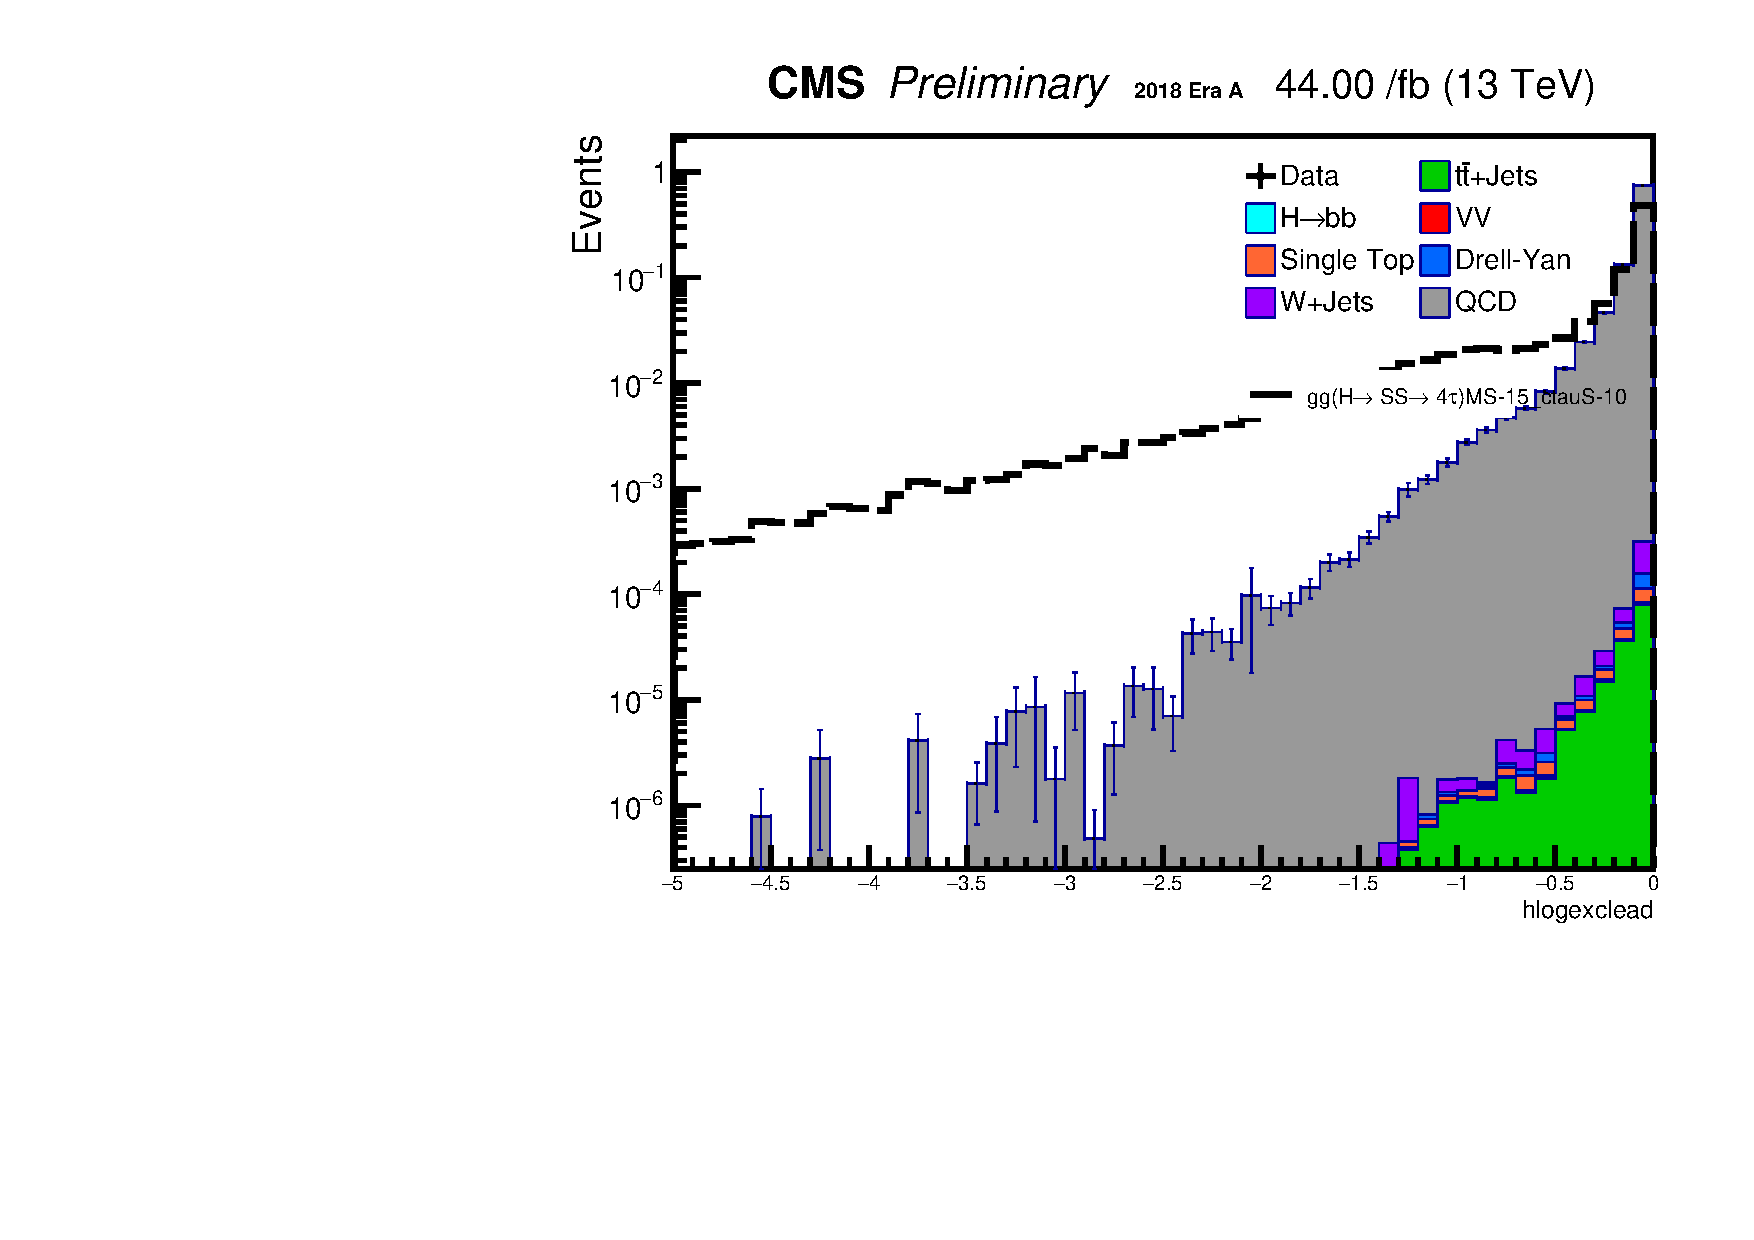
\includegraphics[width=0.47\linewidth]{figs/log_AnalysisNote_MS-15_ctauS-10_hlogexclead.pdf}
   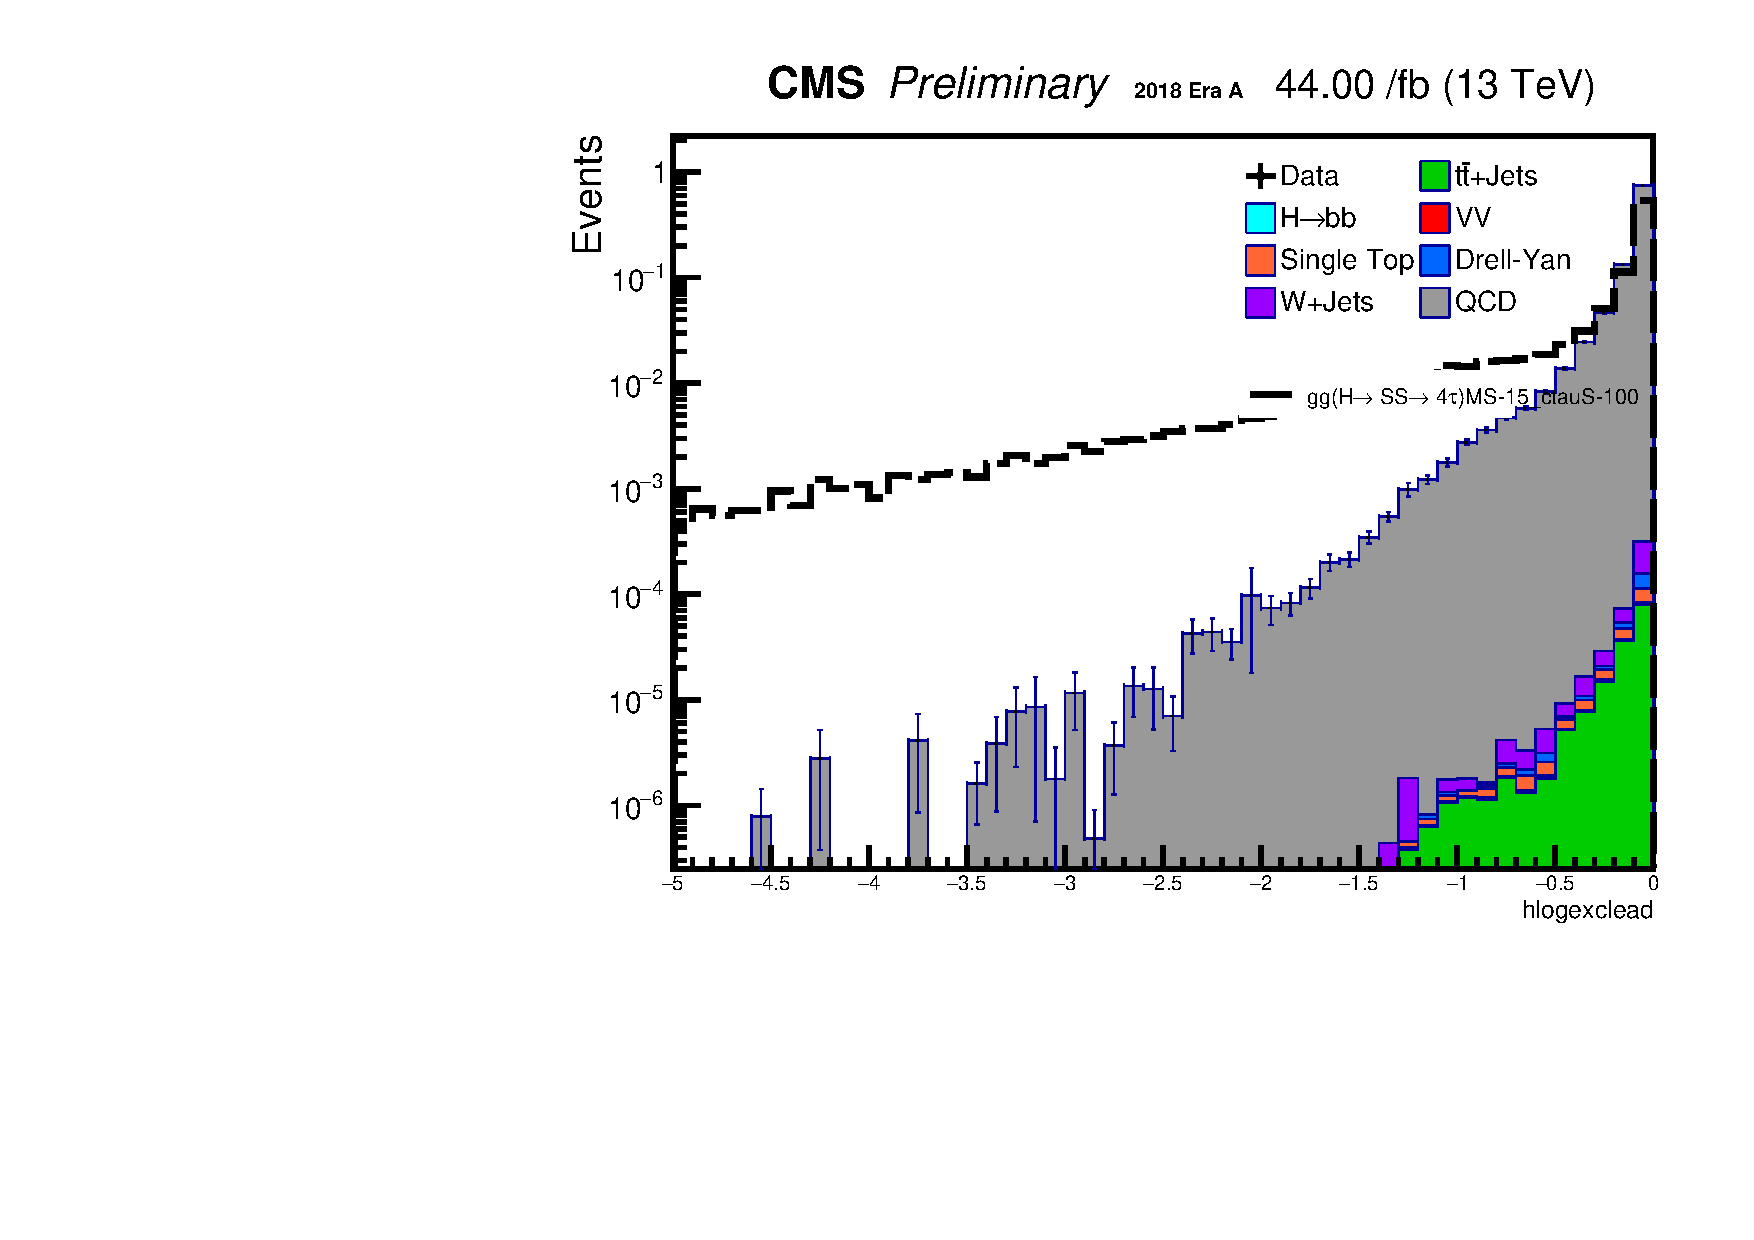
\includegraphics[width=0.47\linewidth]{figs/log_AnalysisNote_MS-15_ctauS-100_hlogexclead.pdf}
   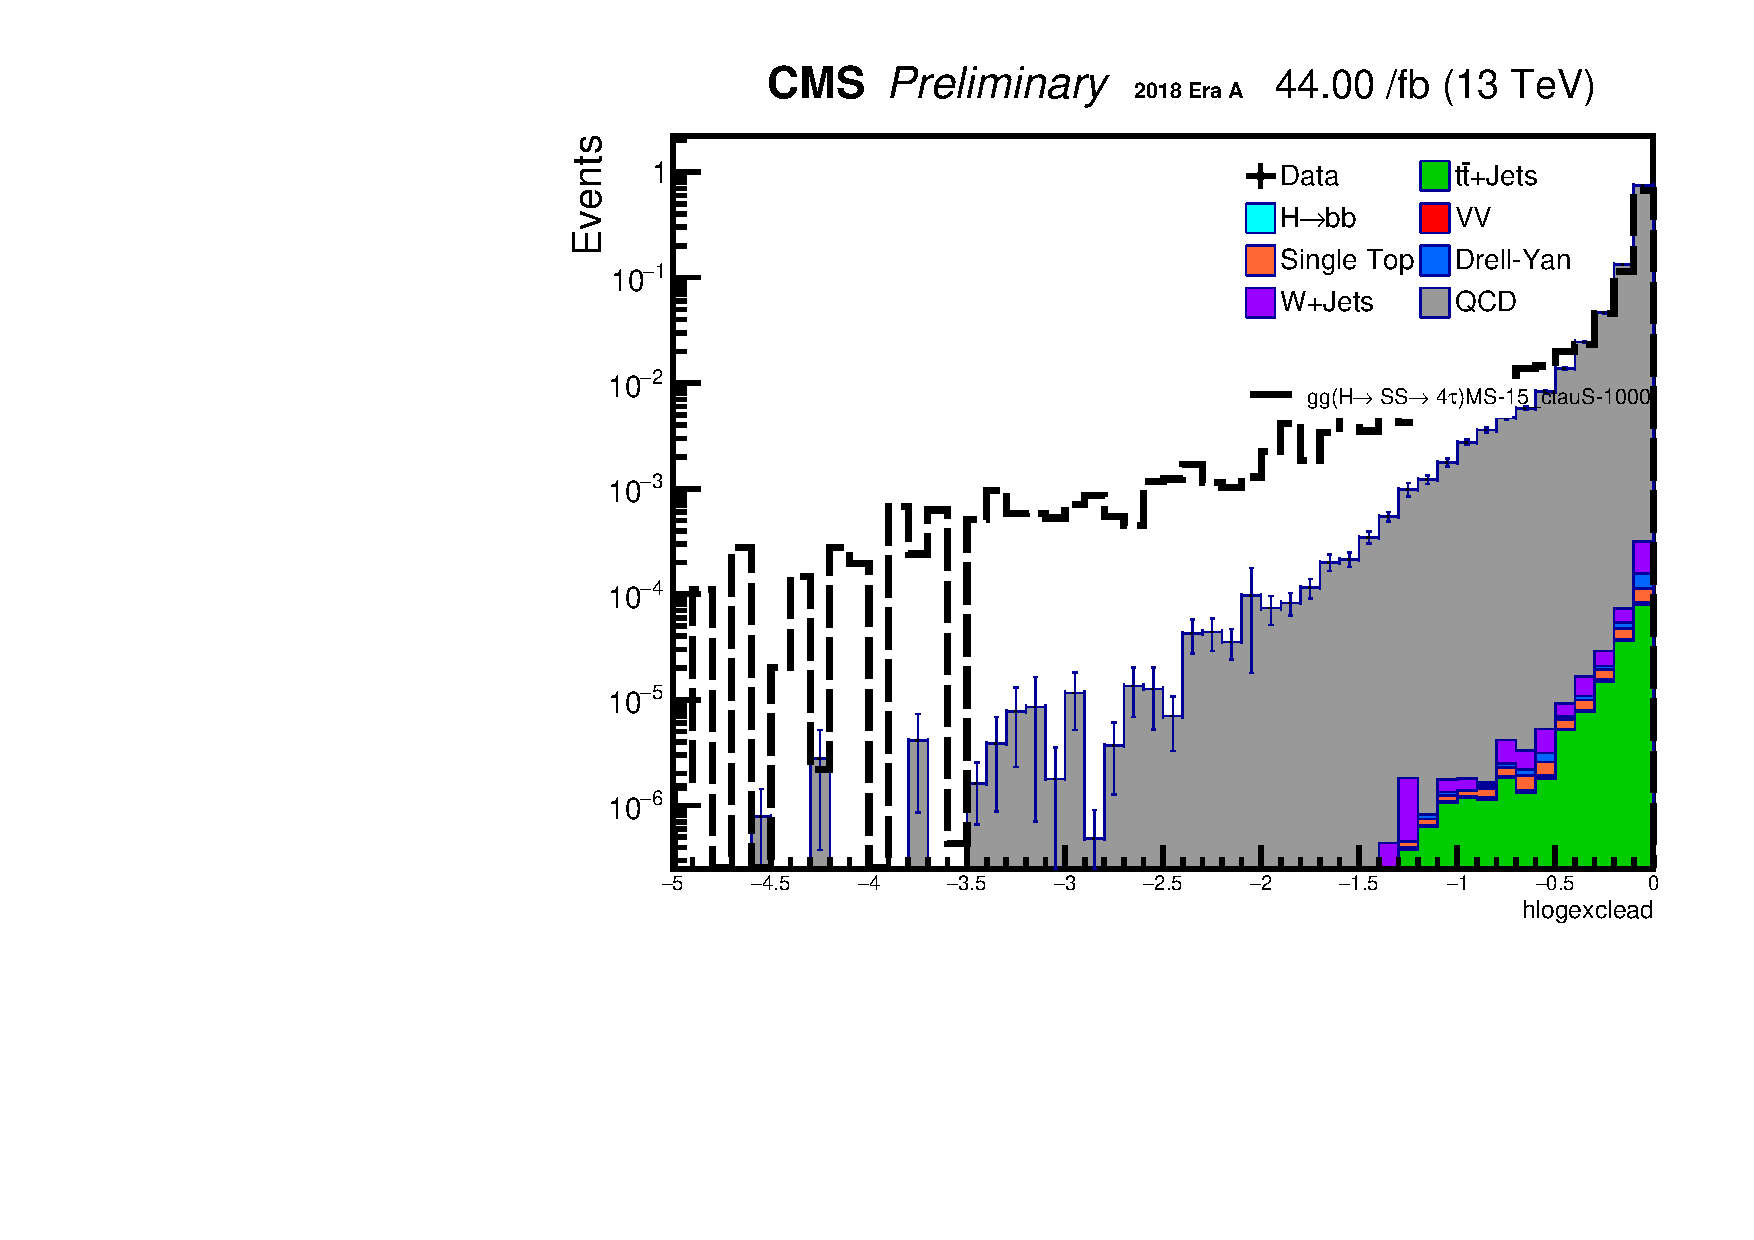
\includegraphics[width=0.47\linewidth]{figs/log_AnalysisNote_MS-15_ctauS-1000_hlogexclead.pdf}
   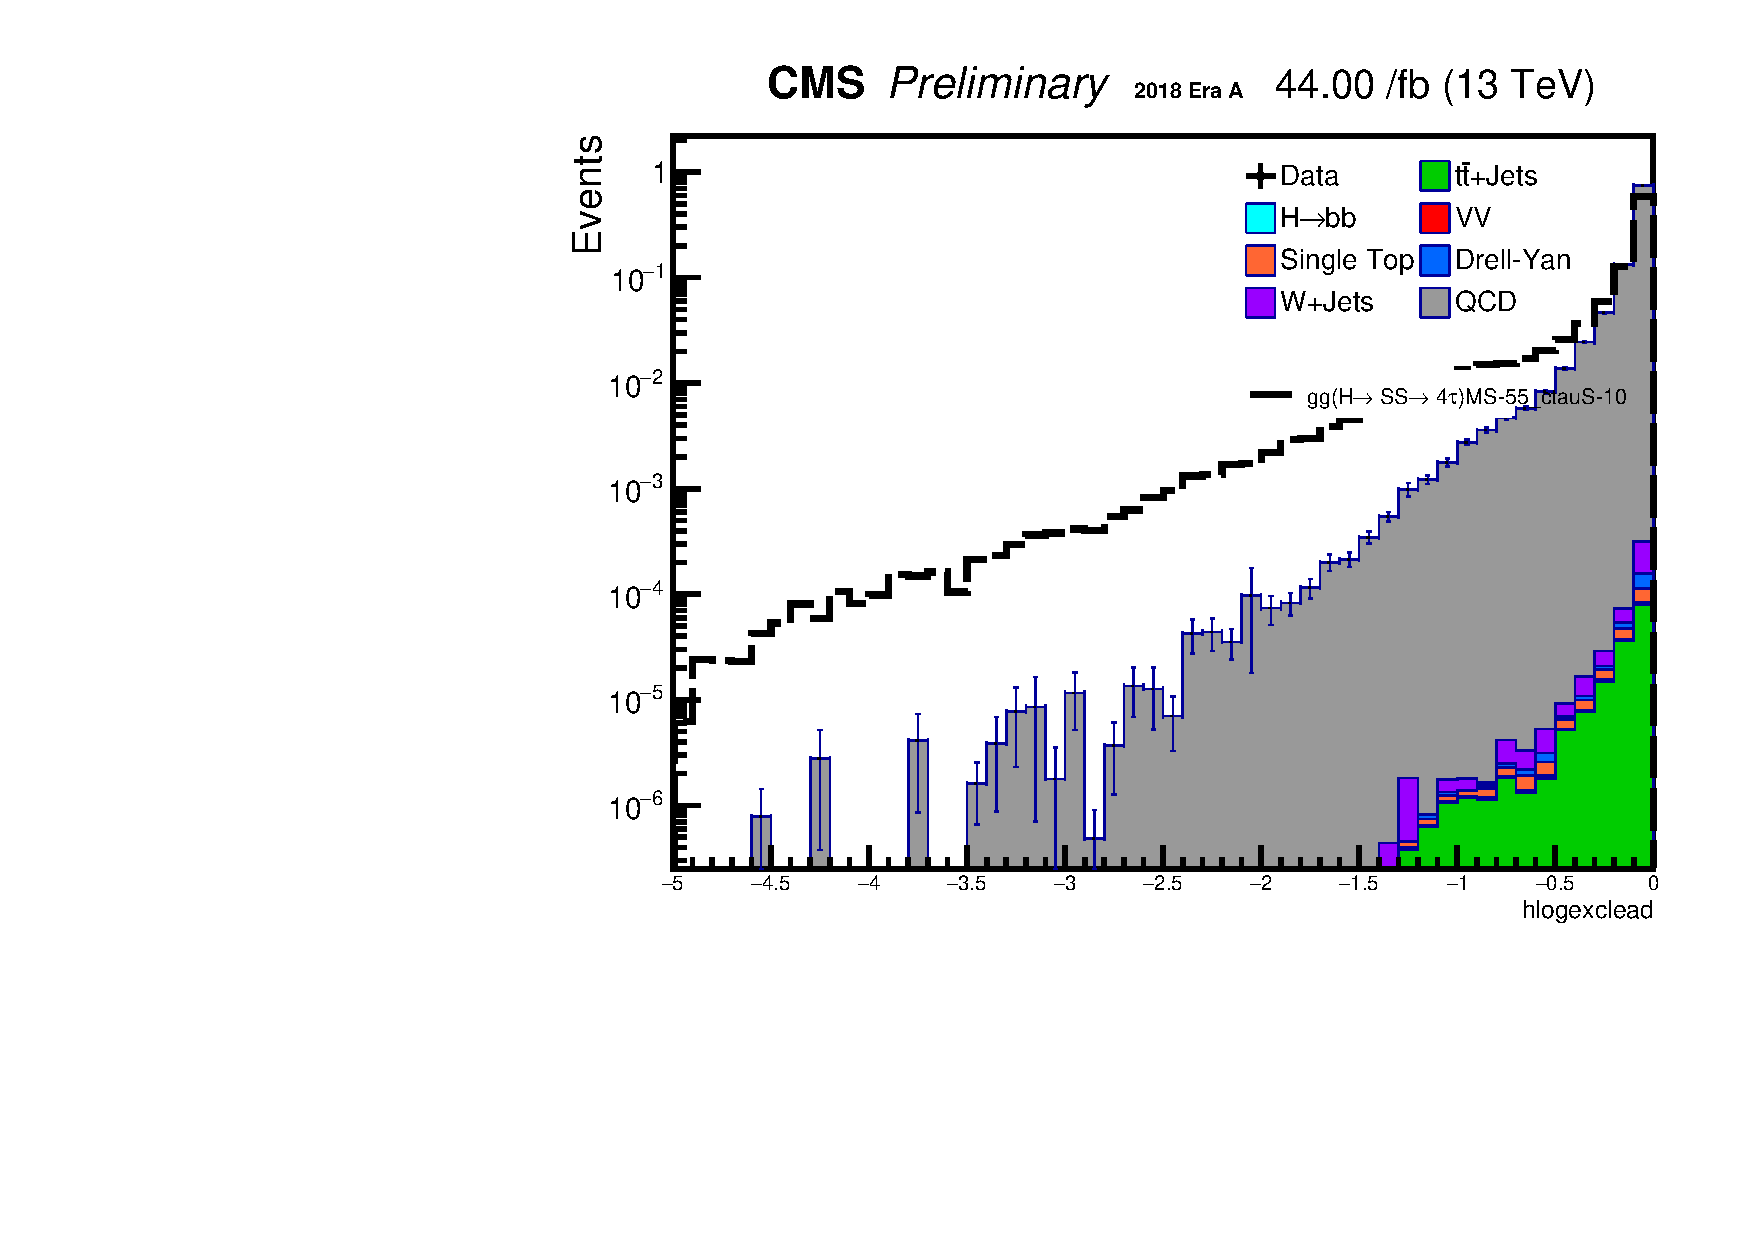
\includegraphics[width=0.47\linewidth]{figs/log_AnalysisNote_MS-55_ctauS-10_hlogexclead.pdf}
 \end{figure}

\begin{figure}[h!]
  \caption{Data/MC agreement for loglead and logexclead scores}
  \label{fig:DataMCscore}
  \centering
  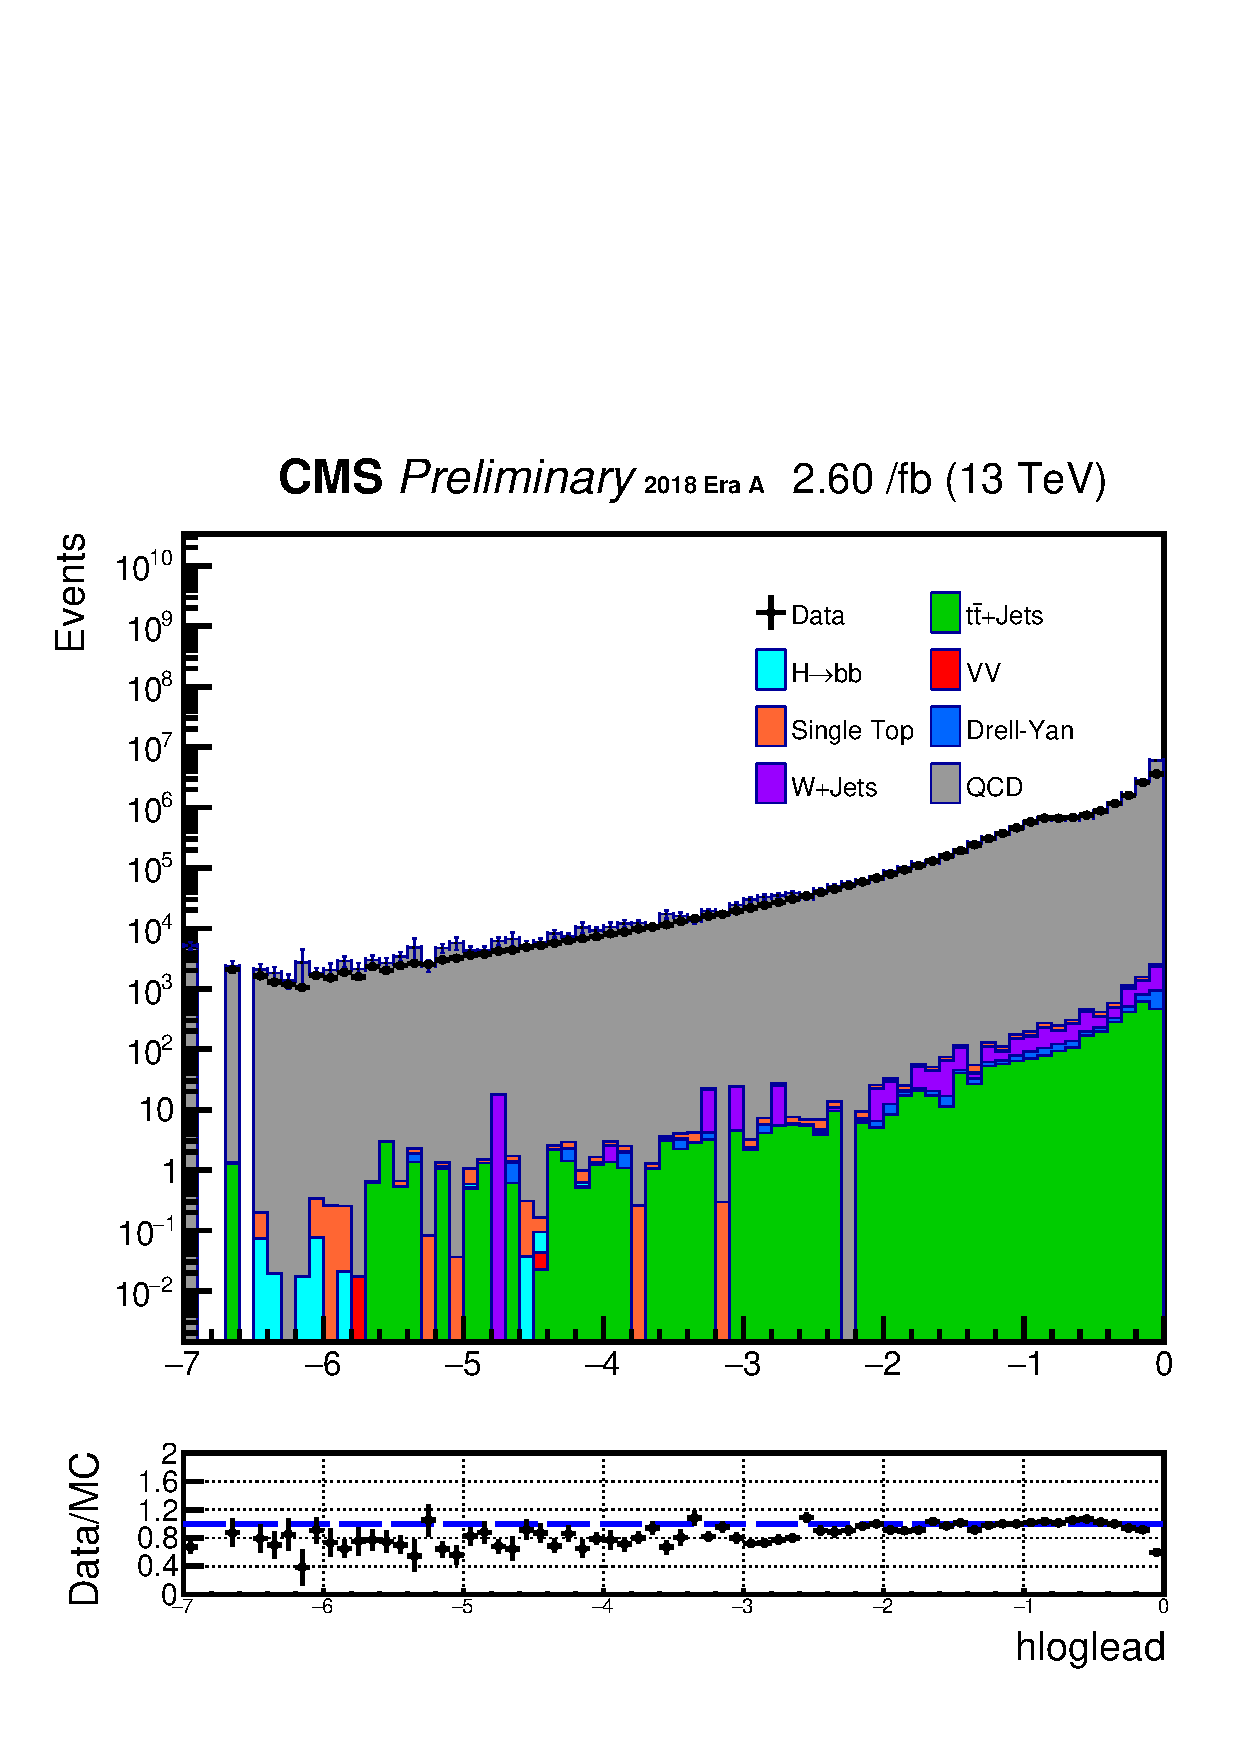
\includegraphics[width=0.67\linewidth]{figs/Data_log_AnalysisNote_MS-15_ctauS-10_hloglead.pdf}
  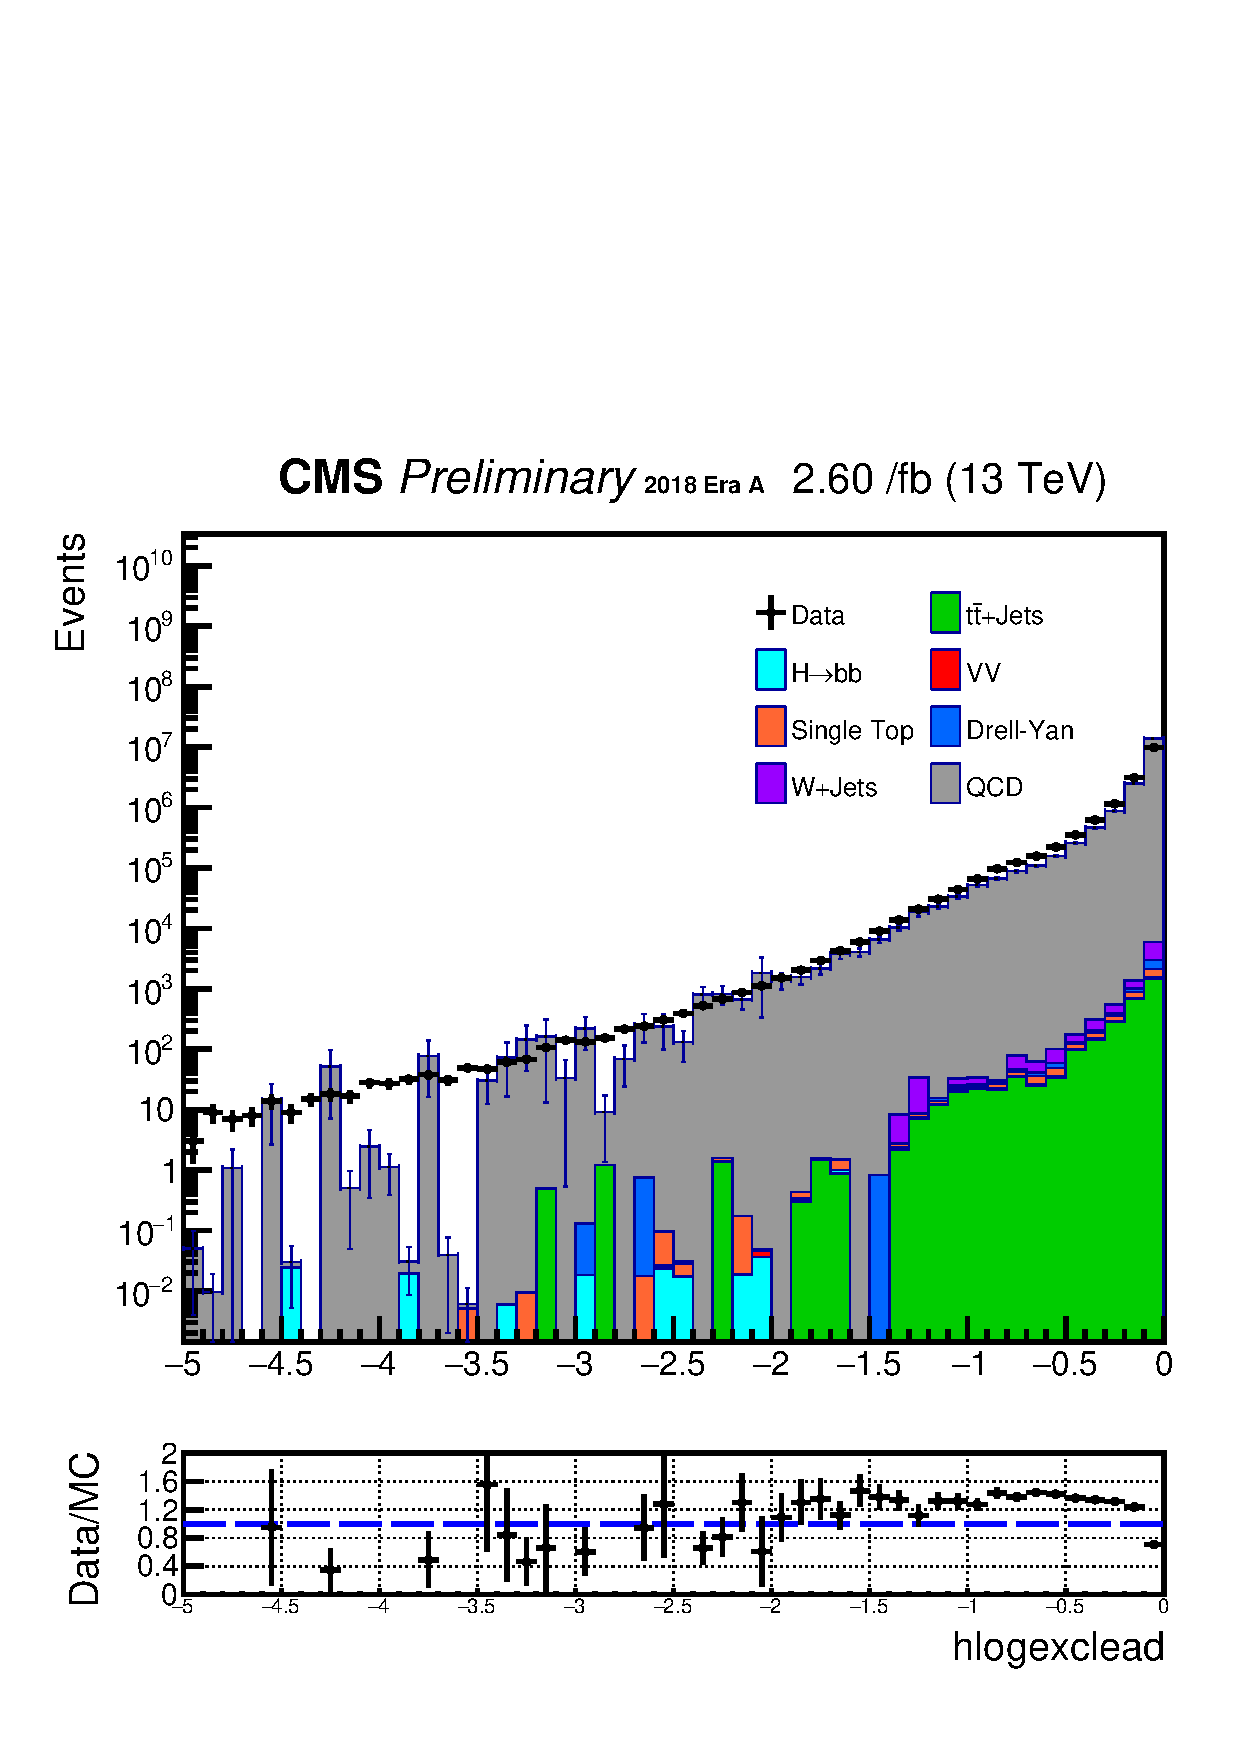
\includegraphics[width=0.67\linewidth]{figs/Data_log_AnalysisNote_MS-15_ctauS-10_hlogexclead.pdf}
\end{figure}

\begin{figure}[h!]
  \caption{Data/MC agreement for leading and subleading ROI distributions}
  \label{fig:DataMCscore2}
  \centering
  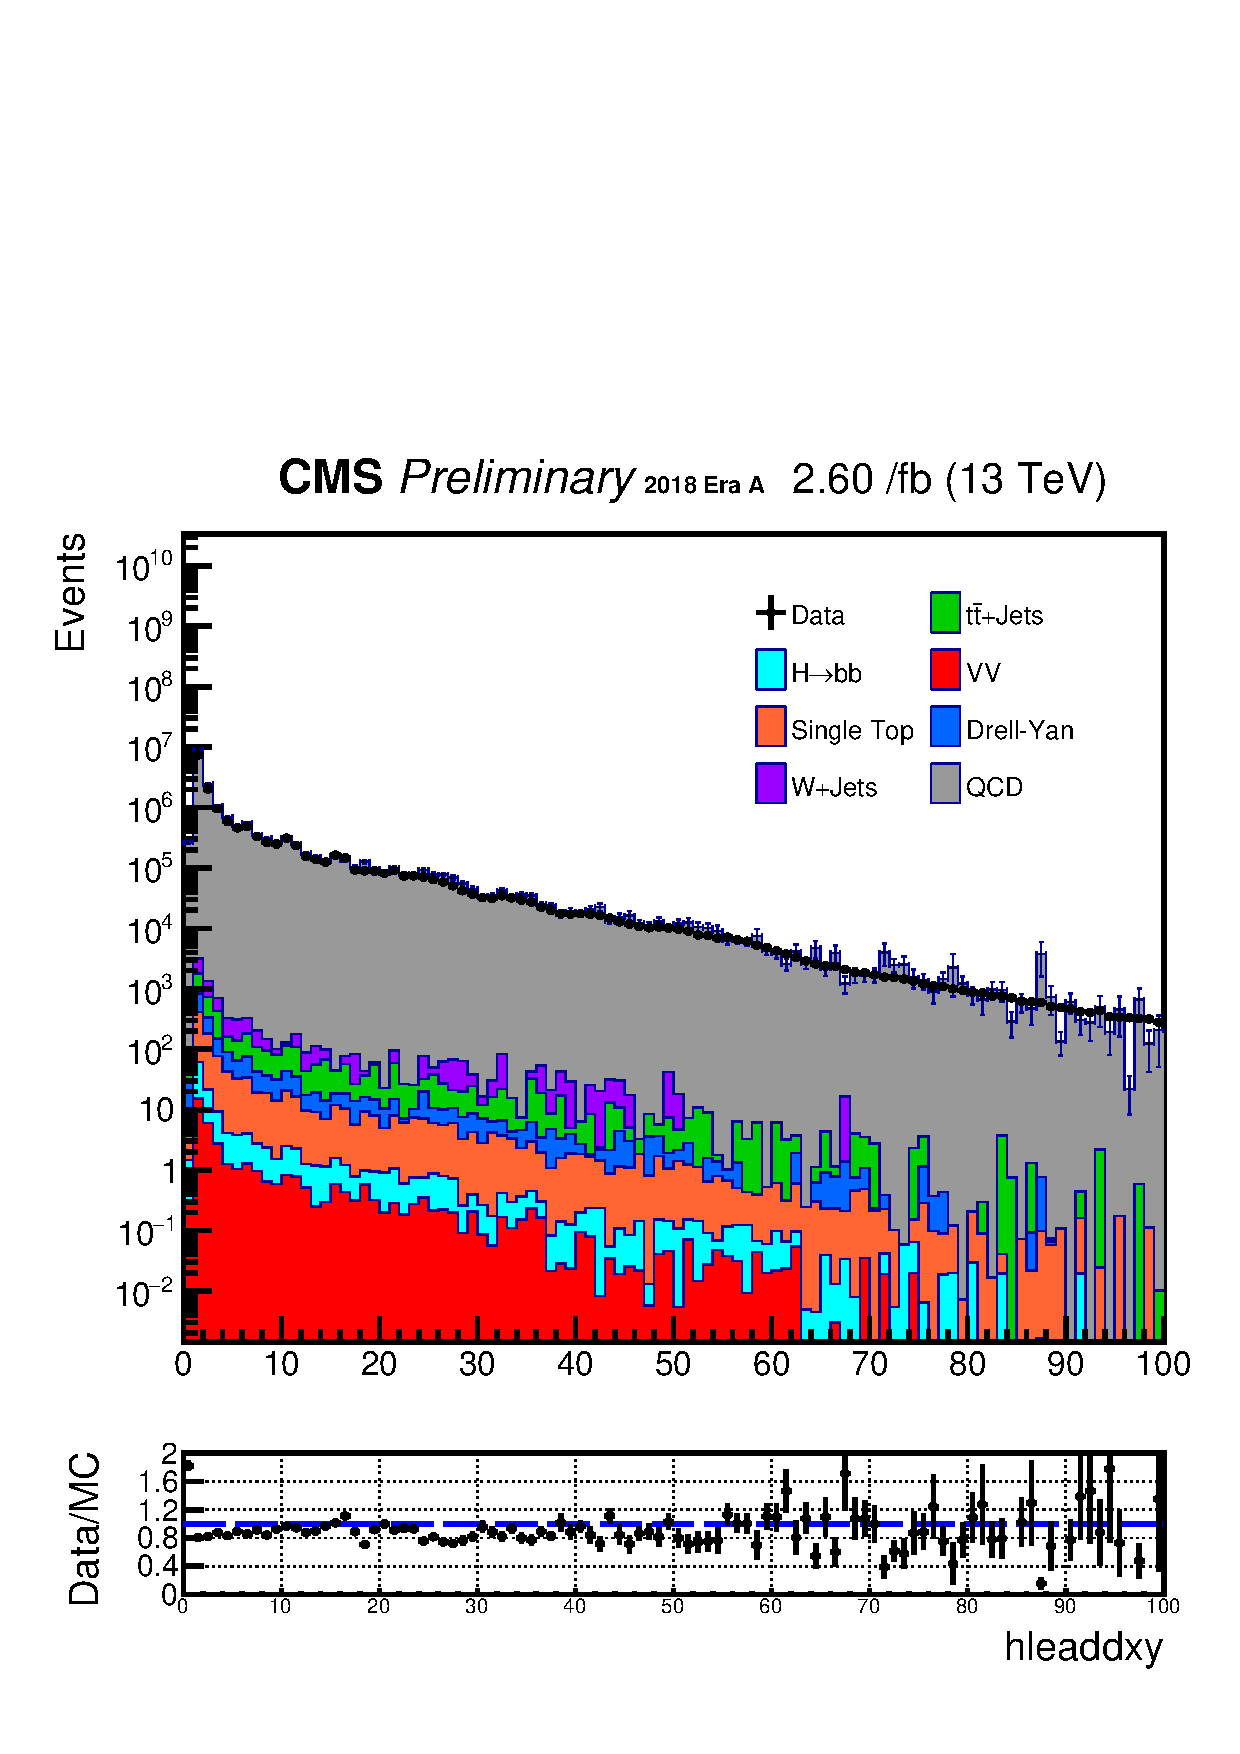
\includegraphics[width=0.57\linewidth]{figs/Data_log_AnalysisNote_MS-15_ctauS-10_hleaddxy.pdf}
  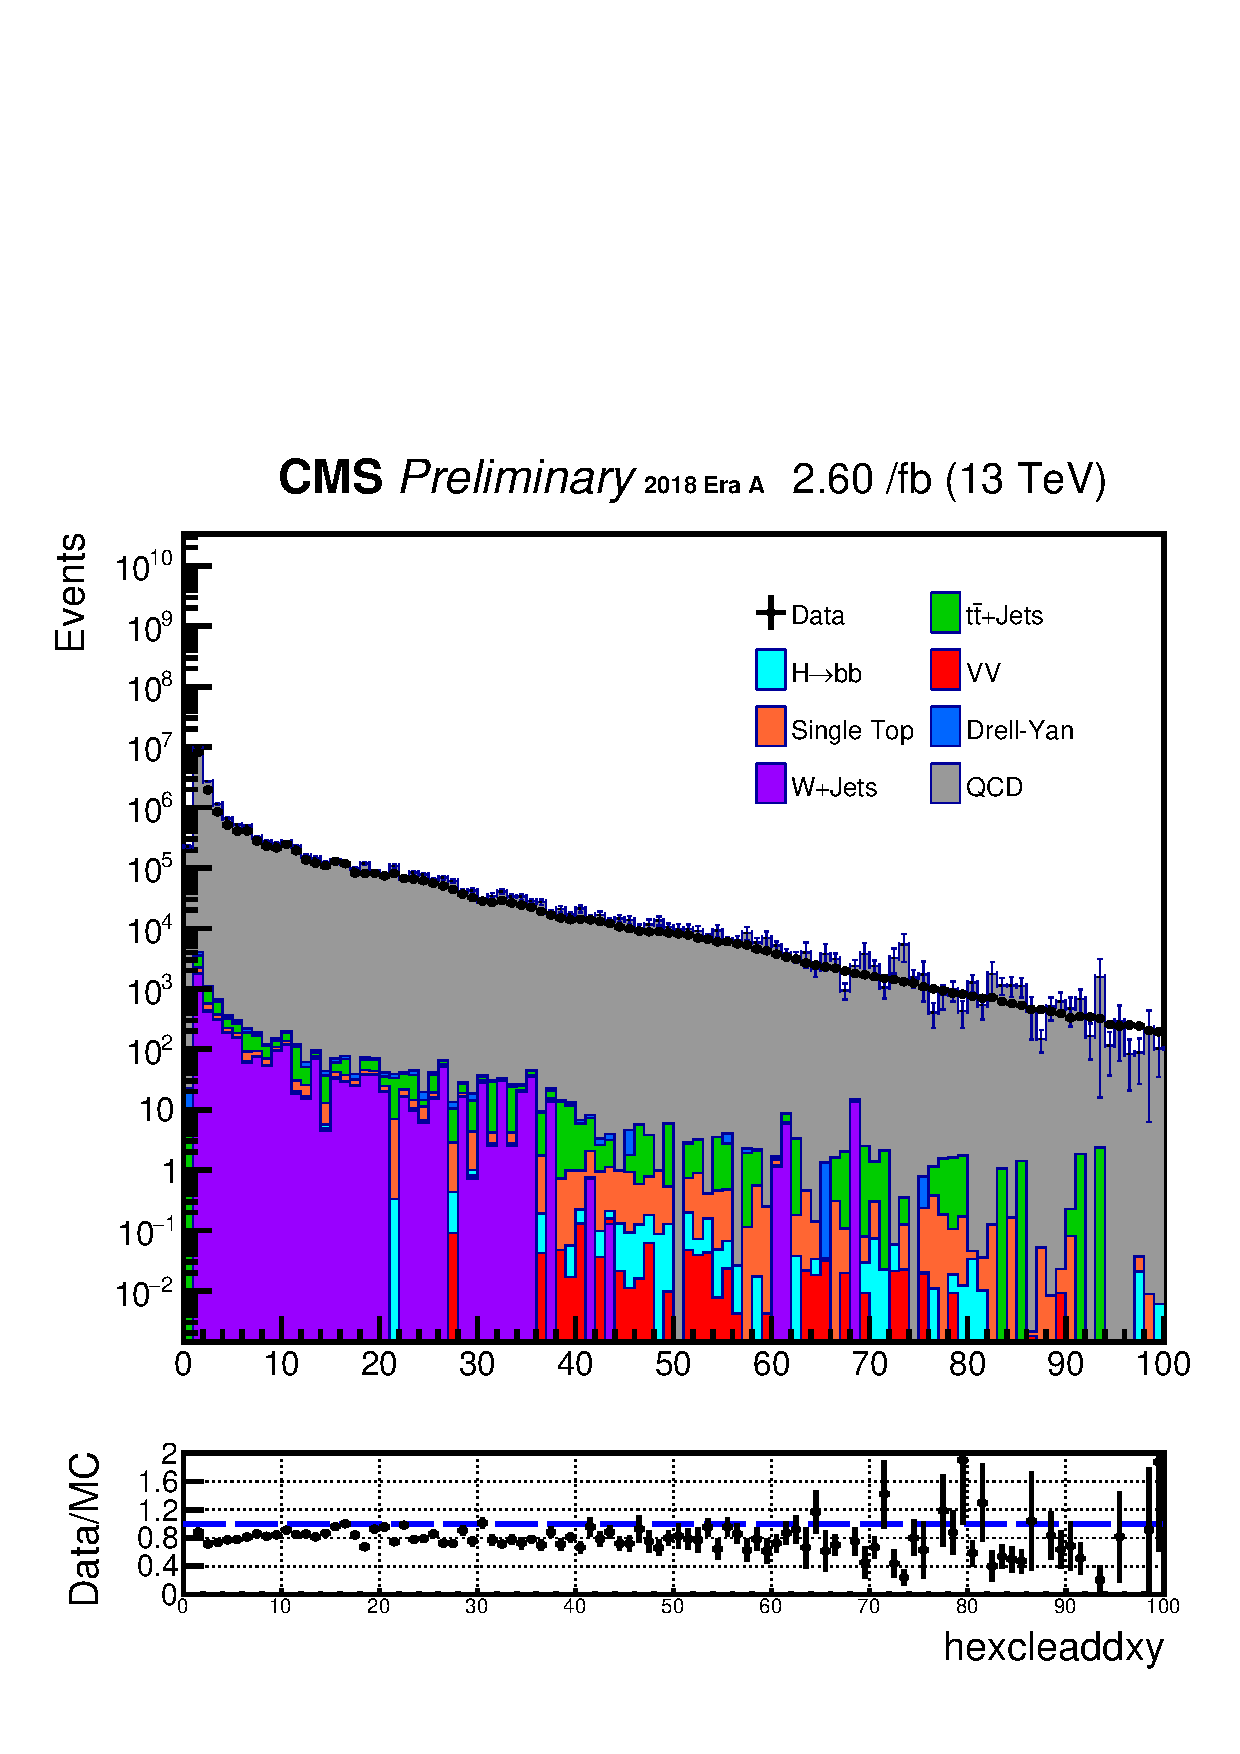
\includegraphics[width=0.57\linewidth]{figs/Data_log_AnalysisNote_MS-15_ctauS-10_hexcleaddxy.pdf}

\end{figure}


\begin{figure}[h!]
  \caption{Data/MC agreement for leading and subleading ROI distributions}
  \label{fig:DataMCscore3}
  \centering
  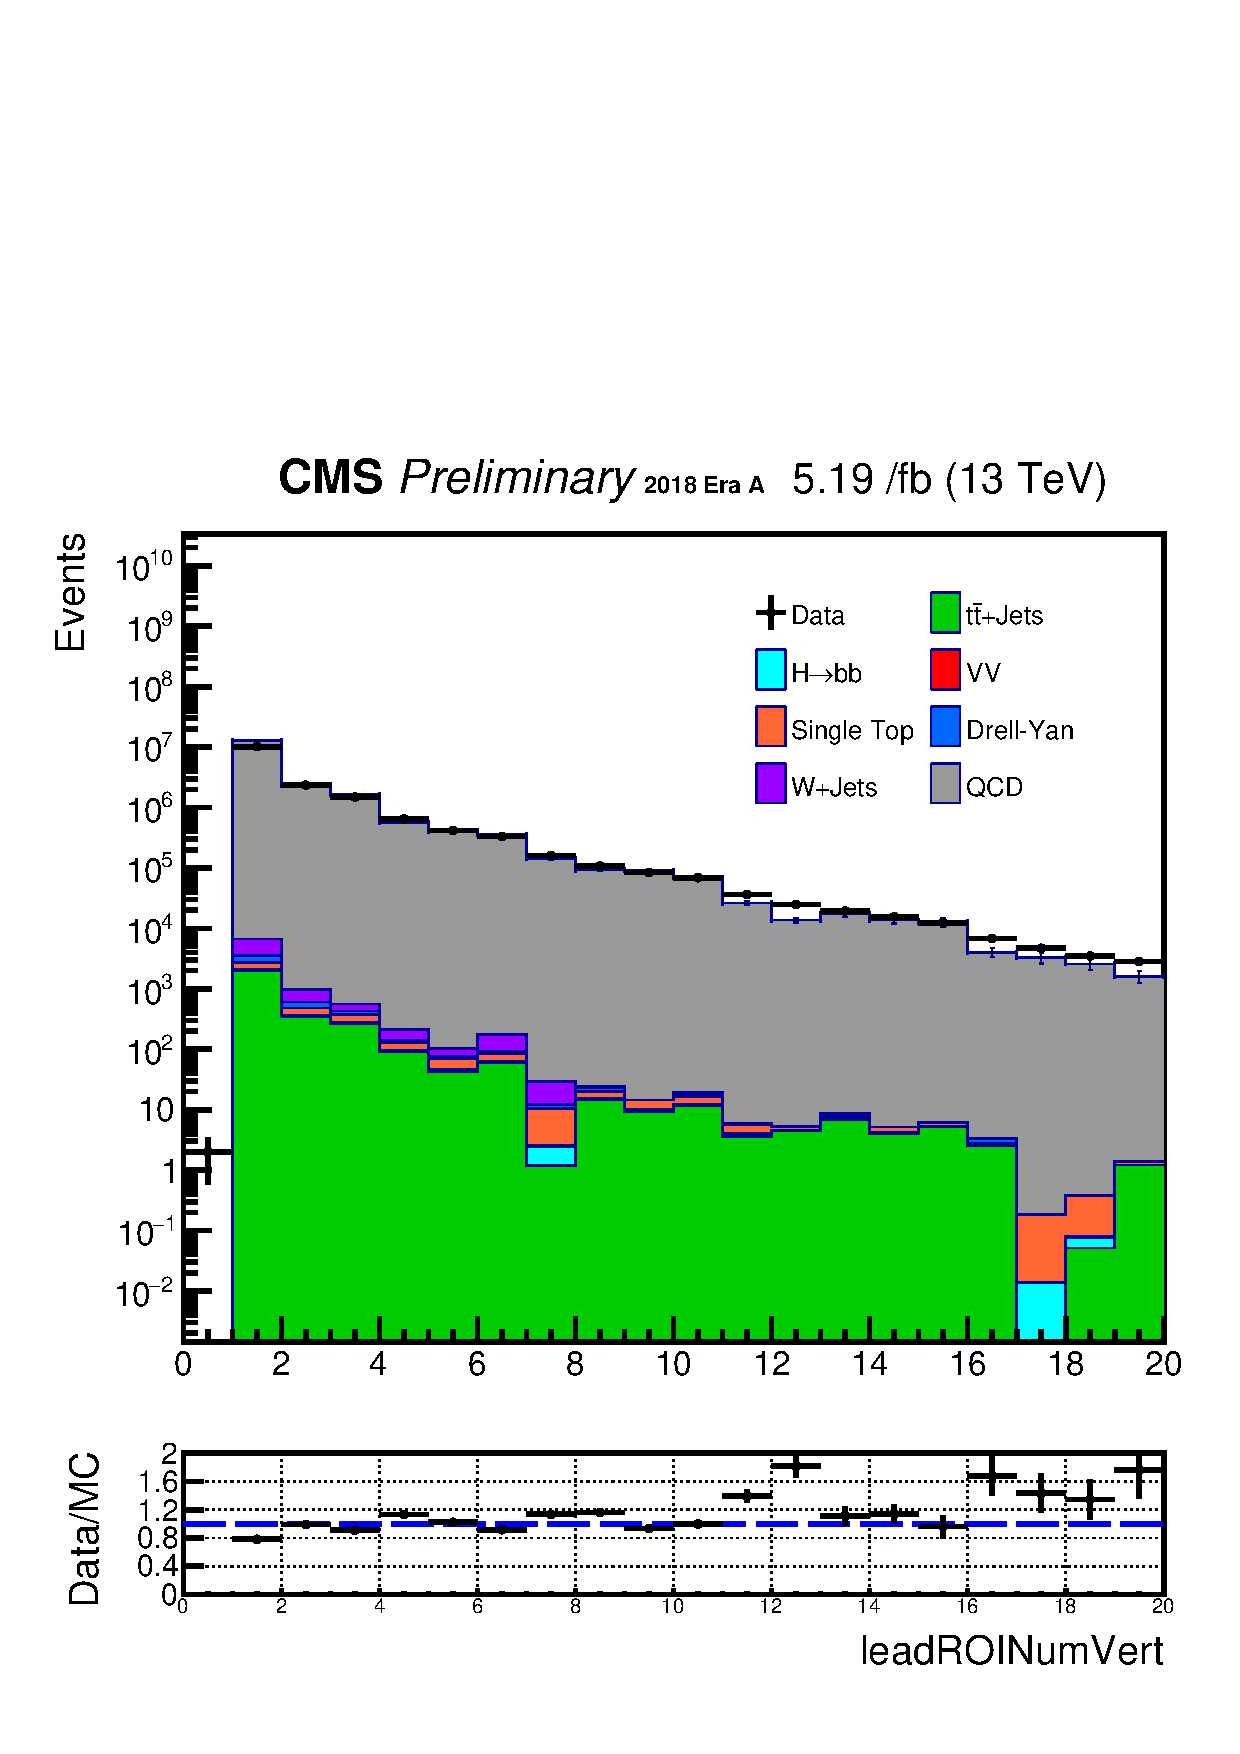
\includegraphics[width=0.57\linewidth]{figs/Data_log_AnalysisNote_MS-15_ctauS-10_leadROINumVert.pdf}
  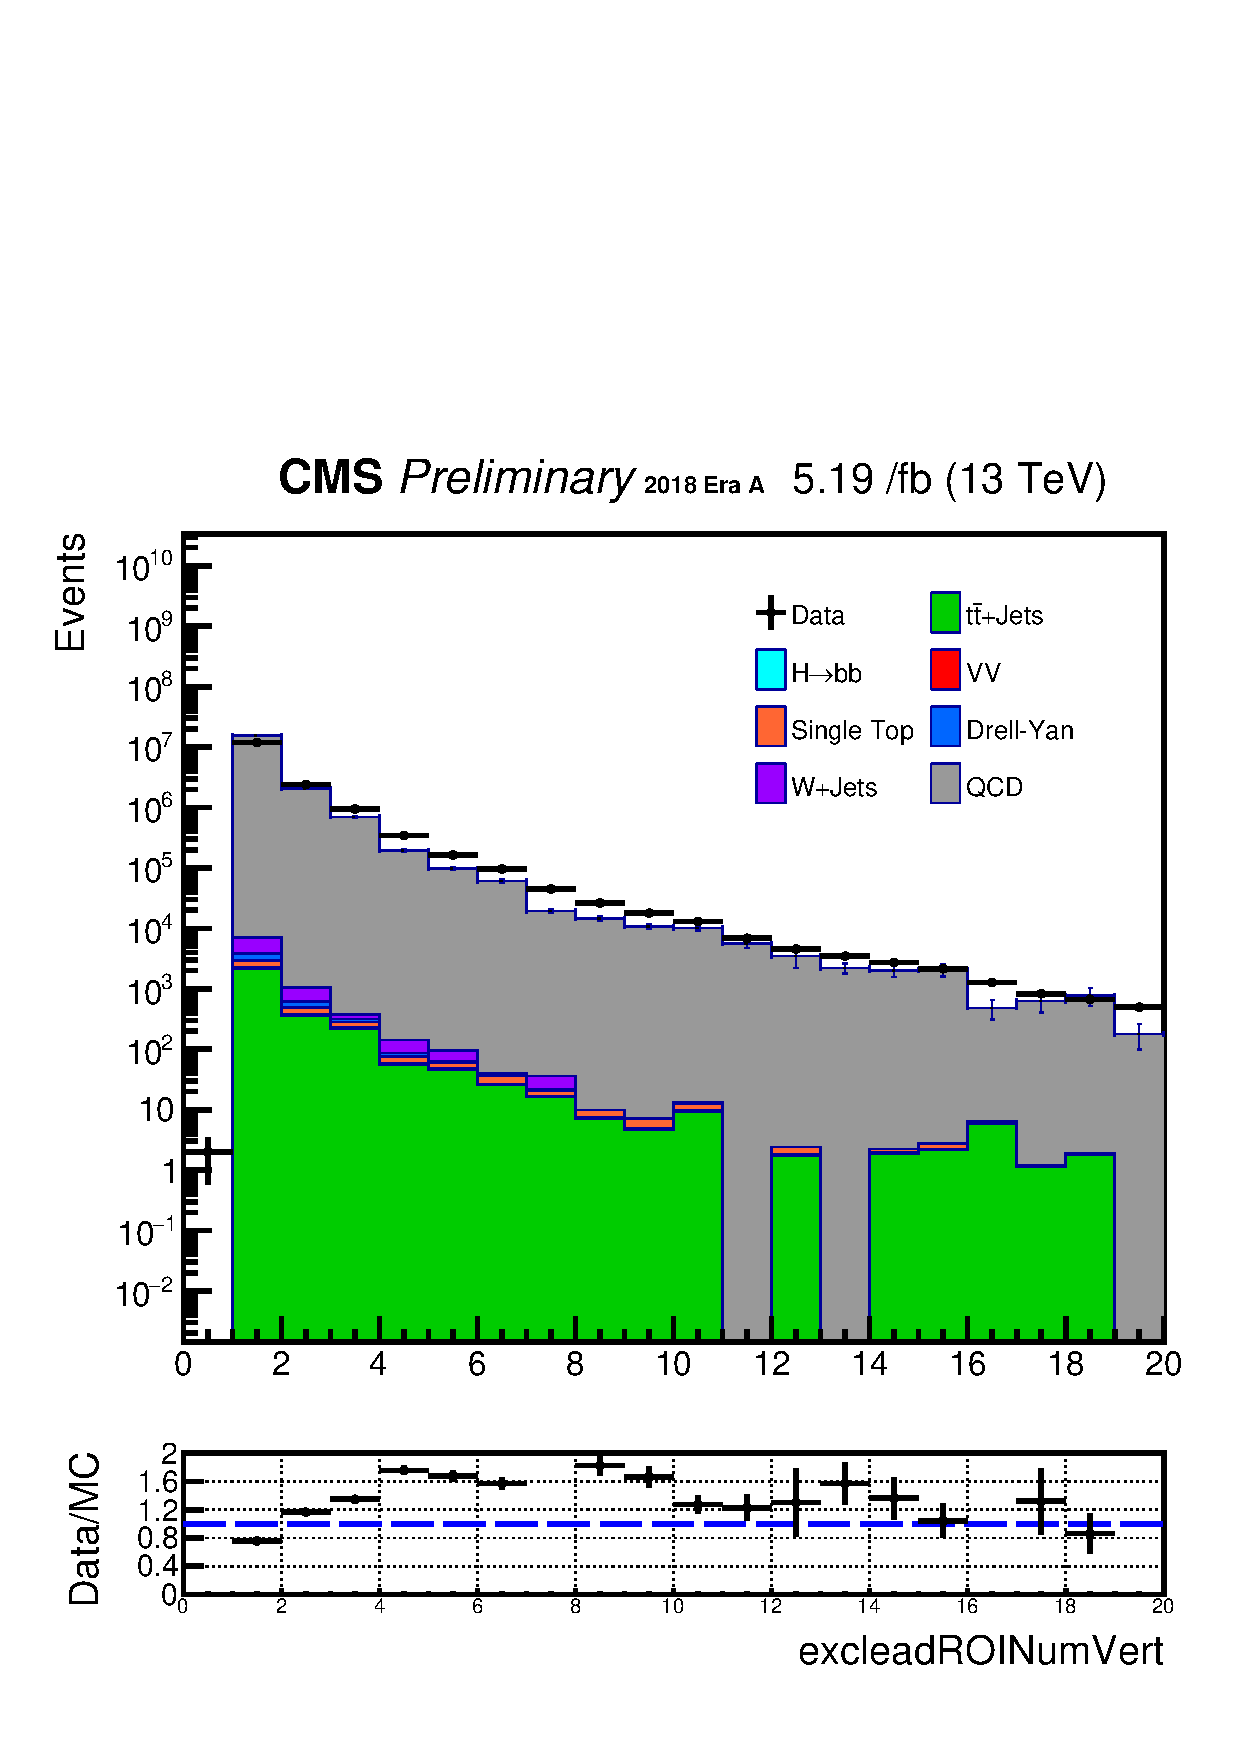
\includegraphics[width=0.57\linewidth]{figs/Data_log_AnalysisNote_MS-15_ctauS-10_excleadROINumVert.pdf}
\end{figure}


\begin{figure}[h!]
  \caption{Data/MC agreement for leading and subleading ROI distributions}
  \label{fig:DataMCscore4}
  \centering
  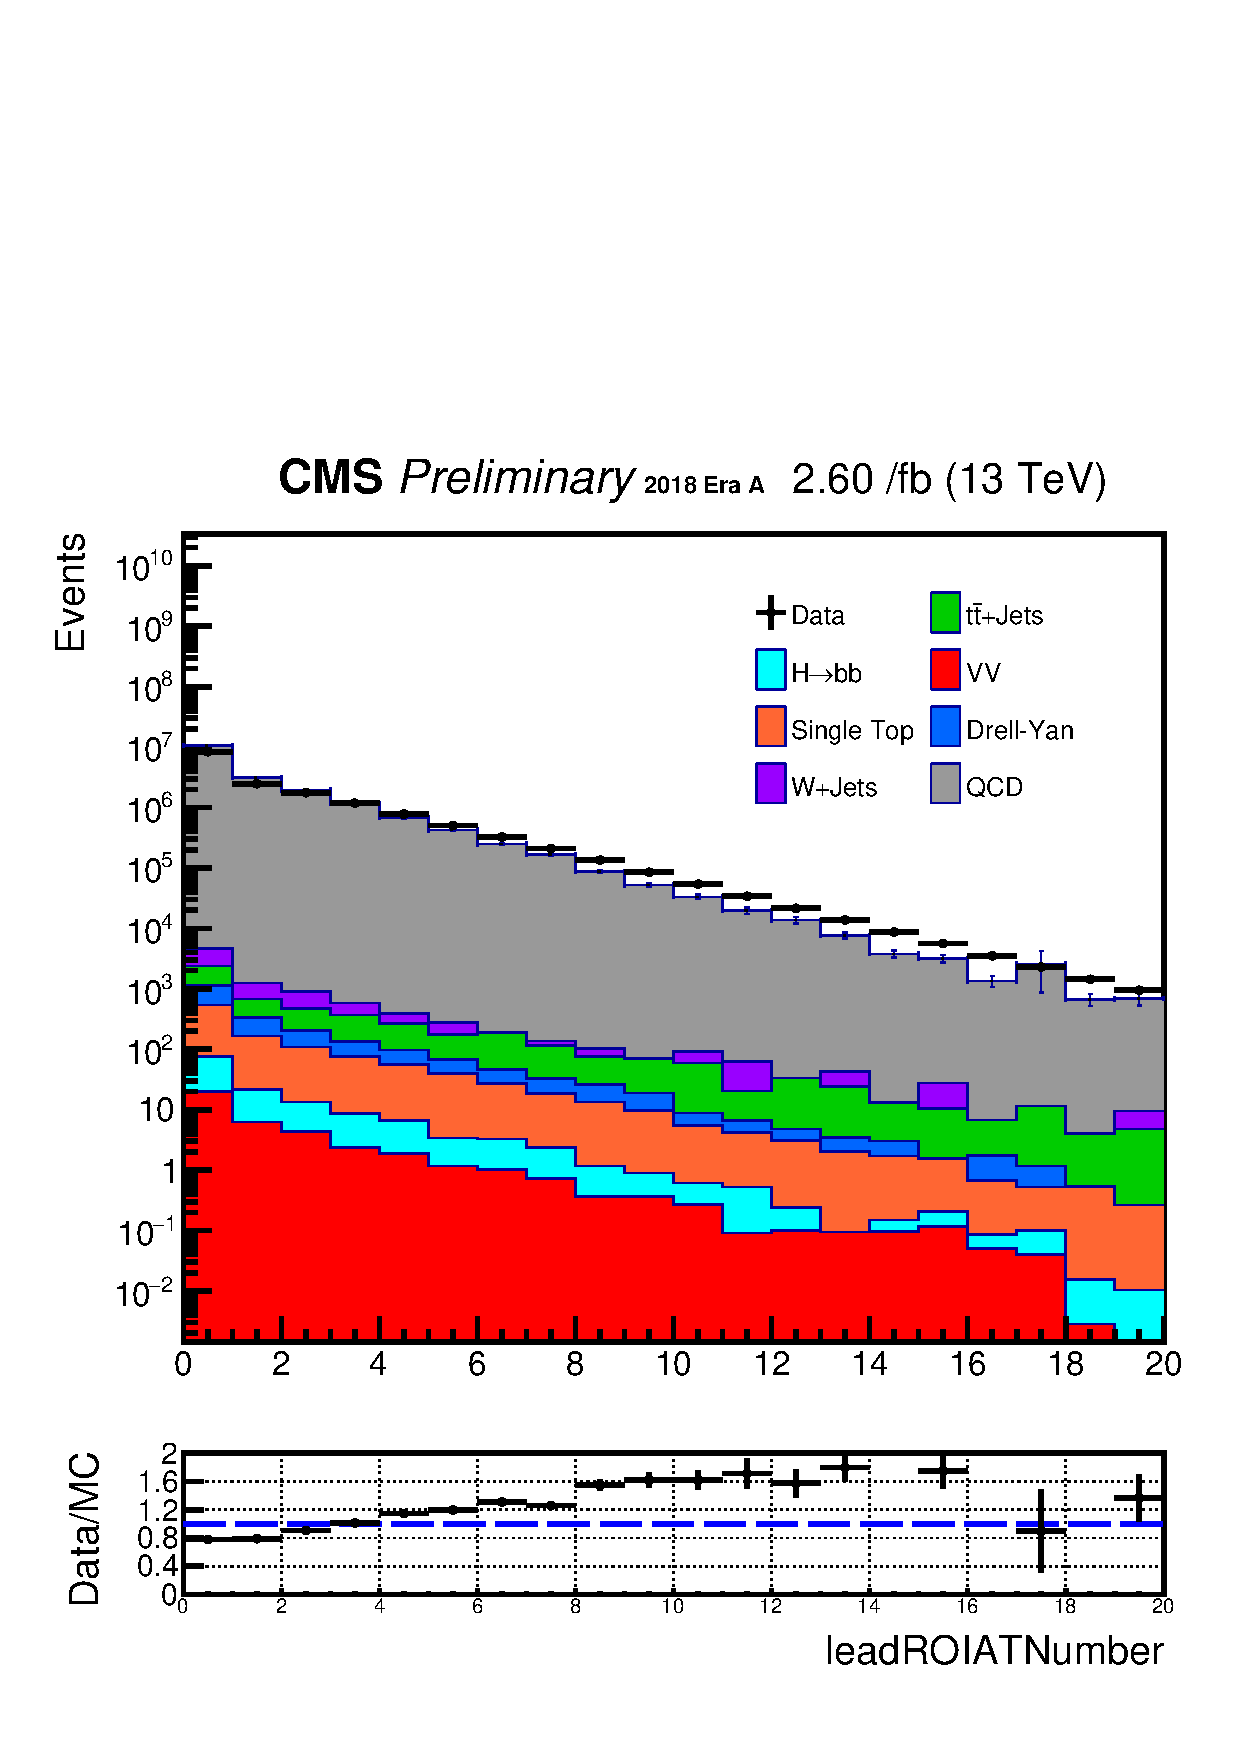
\includegraphics[width=0.57\linewidth]{figs/Data_log_AnalysisNote_MS-15_ctauS-10_leadROIATNumber.pdf}
  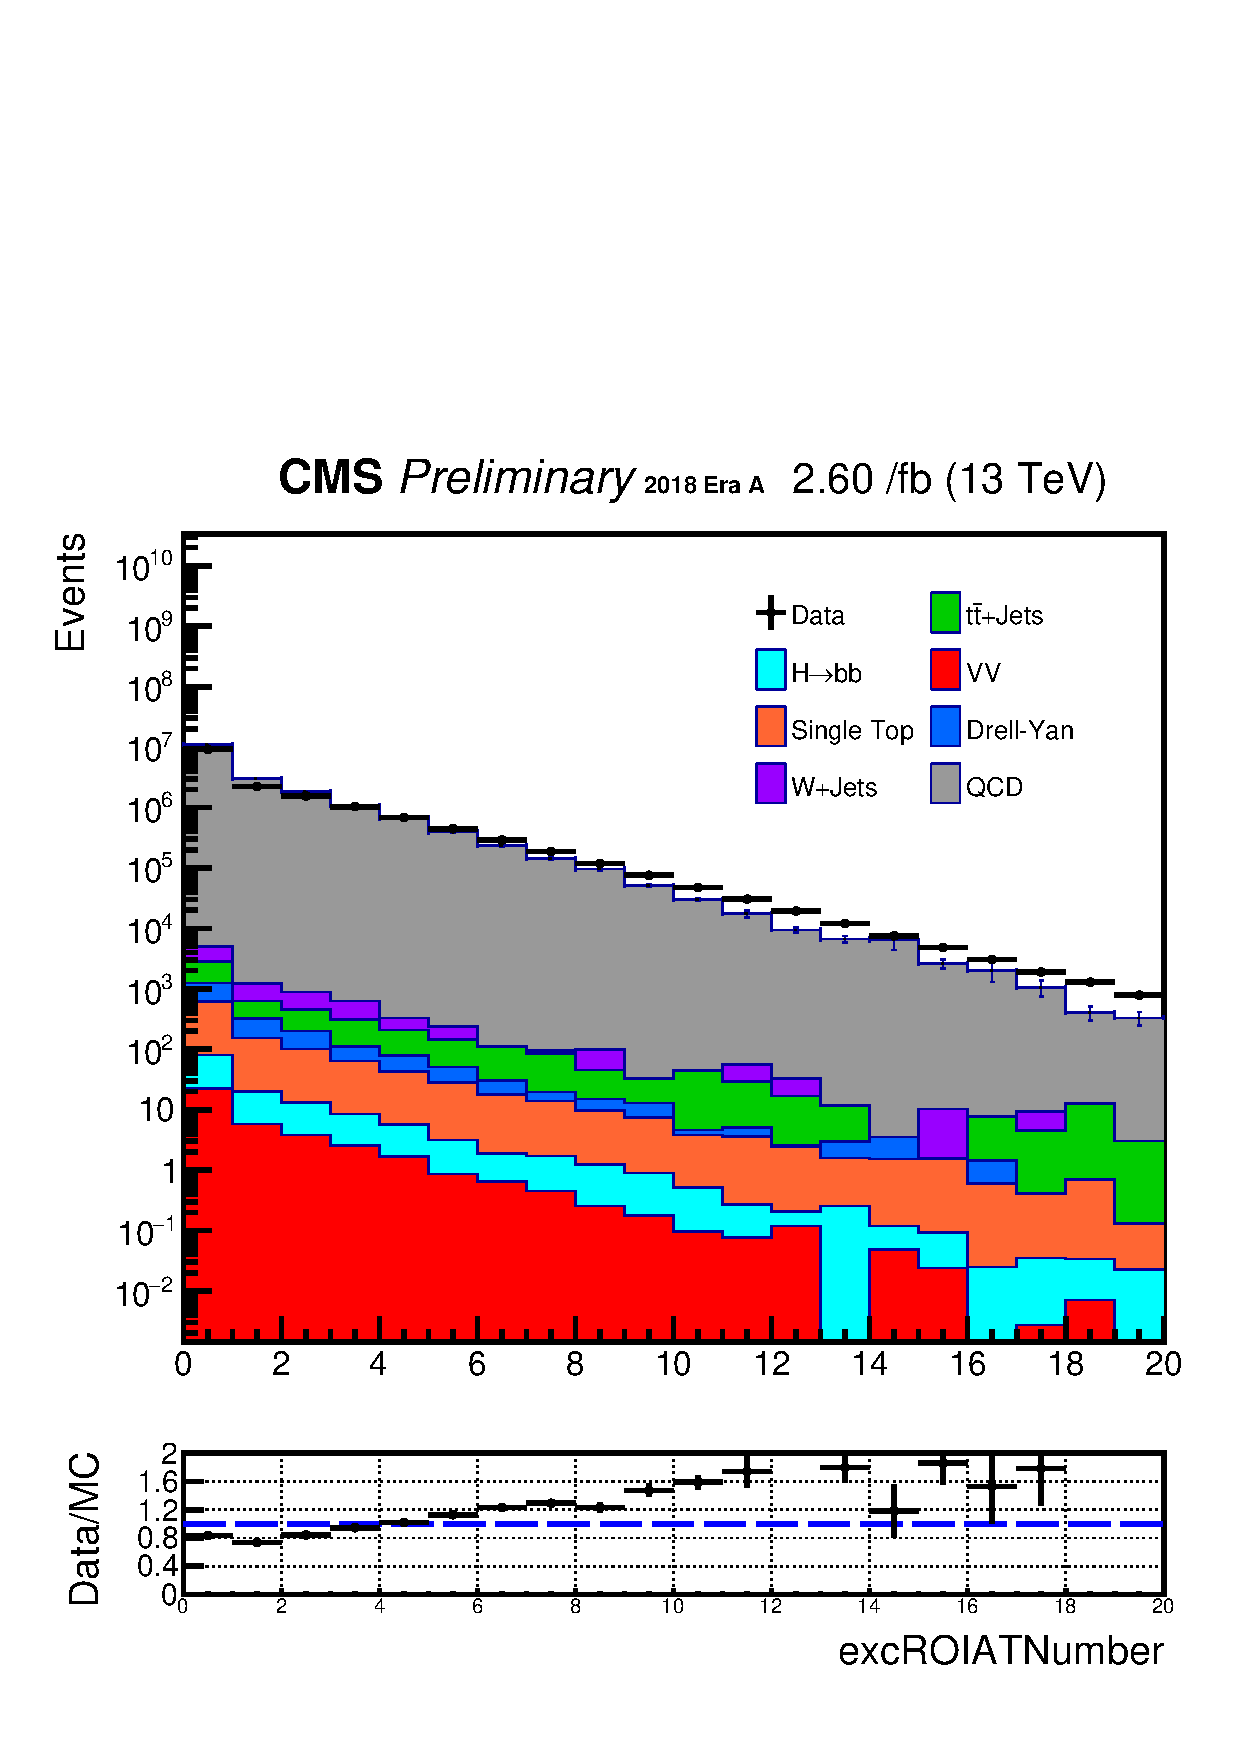
\includegraphics[width=0.57\linewidth]{figs/Data_log_AnalysisNote_MS-15_ctauS-10_excROIATNumber.pdf}

\end{figure}

